    \documentclass{article}

\usepackage[english]{babel}
\usepackage{amsmath}
% Set page size and margins
% Replace `letterpaper' with `a4paper' for UK/EU standard size
\usepackage[letterpaper,top=2cm,bottom=2cm,left=2cm,right=2cm,marginparwidth=1.75cm]{geometry}
\usepackage{subcaption}
% Useful packages
\usepackage{amsmath}
\usepackage{graphicx}
\usepackage[colorlinks=true, allcolors=blue]{hyperref}
\usepackage{natbib} % 常用的引用宏包,支持多种样式,包括类似APA的
% \usepackage{apacite} % 专门的APA样式宏包



\title{MATH285 Lab Report}
\author{Yuan Shihong , Li Binghe , Wang Chenyi, Zhang Kerui, Xia Wubing}

\begin{document}


\begin{titlepage}
    \centering
    \vspace*{2cm}
    
    \Huge
    \textbf{ZJU-UIUC INSTITUTE}
    
    \vspace{0.5cm}
    \LARGE
    SP25 MATH285 Lab Report
    
    \vspace{1.5cm}
    
    \Large
    Group 10 Members:
    
    \vspace{0.5cm}
    \begin{minipage}{0.6\textwidth}
    \centering
    \begin{tabbing}
    Yuan Shihong \hspace{2cm} \= 3230116076 \\
    Wang Chenyi \> 3230110995 \\
    Zhang Kerui \> 3230111488 \\
    Xia Wubing \> 3230110985 \\
    Li Binghe \> 3230116075 \\
    \end{tabbing}
    \end{minipage}

    \vspace{2cm}
    
    \Large
    \textbf{HONOR STATEMENT}
    
    \vspace{0.5cm}
    
    \normalsize
    We declare that this report is our own original work. For its preparation, we have not used any other resources than those cited as references. Every group member has a fair share in this work.
    
    \vspace{2cm}
    
    \begin{flushleft}
    \large
    Sign:
    
    \vspace{1.5cm}
    
    Date: 2025.5.25
    \end{flushleft}



    
\end{titlepage}


\maketitle
%%%%%%%%%%%%%%%%%%%%%%%%%%%%%%%%%%%%%%%%%%%%%%%%%%%%%%%%%%%%%%%%%%%%%%%%%%%%%%%%%%%%%%%%%%%%%%%%%%%%% 








\begin{abstract}

This lab report aims to investigate the maximal solutions and their domains for two initial value problems (IVPs) using both numerical and analytical methods. The specific problems are as follows: 

\begin{equation*}
    \text{(IVP1)} \quad y' = t^3 +y^3, \quad y(0) = -1
\end{equation*}
\begin{equation*}
    \text{(IVP2)} \quad y' = t^3 +y^3, \quad y(0) = 0
\end{equation*}
\begin{equation*}
    \text{(IVP3)} \quad y' = t^3 +y^3, \quad y(0) = 1
\end{equation*}
\end{abstract}

\section{Introduction}


This experiment focuses on solving three initial value problems (IVPs) using numerical methods such as Euler, Improved Euler, and Runge-Kutta and Power Series.


\textbf{Specifically, we determined the following for the solution's domain and behavior based on the initial condition $y_0$:}

\begin{itemize}
    \item When \textbf{$y_0 = -1$}, the function's domain extends from $-\infty$ to approximately \textbf{0.502}. The graph of the solution exhibits a shape similar to a ``check mark'' (or a hyperbola-like curve with two branches).
    \item When \textbf{$y_0 = 0$}, the function's domain extends from $-\infty$ to approximately \textbf{1.647}. The solution is strictly monotonically decreasing across its entire domain.
    \item When \textbf{$y_0 = 1$}, the function's domain extends from $-\infty$ to approximately \textbf{0.498}. Similar to the $y_0 = -1$ case, the solution's graph resembles a ``check mark'' shape.
\end{itemize}


\section{Analysis Problem }

\subsection{Euler Method}

\subsubsection{Mathematical Analysis}

The Euler method is a numerical technique for approximating solutions to \( y' = f(t,y) , y(t_0) = y_0\). Here, \(f(t,y) = t^3 + y^3\), and the initial condition is \(y(0) = y_0\). The method uses the iterative formula:
\[y_{n+1} = y_n + h * f(t_n , y_n)\]
\[ t_{n+1} = t_n + h \]
where \( h \) is the step size, \(y_n\) is the numerical solution at \(t_n\).  
\paragraph{Forward in time}(\( t \) increasing): \( t_{n+1} = t_n + h \), \( y_{n+1} = y_n + h (t_n^3 + y_n^3) \).
\paragraph{Backward in time}(\( t \) decreasing): \( t_{n+1} = t_n - h \), \( y_{n+1} = y_n - h (t_n^3 + y_n^3) \).

The mathematical foundation of the Euler method derives from the Taylor series expansion of \( y(t) \) at \( t_n \):
\[
y(t_{n+1}) = y(t_n) + h y'(t_n) + O(h^2)
\]
Neglecting the higher-order term \( O(h^2) \), the Euler method's approximation formula is obtained. The local truncation error is \( O(h^2) \), and the global truncation error is \( O(h) \). 

The stability of the Euler method depends on the step size \( h \) and the properties of the differential equation. For stiff equations, the Euler method may require very small step sizes to remain stable, resulting in significantly increased computational cost.





\subsubsection{Results Display}
Since solutions can blow up (that is, \( |y| \to \infty \)), we iterate until \( |y_n| \) exceeds a large threshold \( M \) (e.g., \( M = 1000 \)), then estimate the blow-up time as the corresponding \( t_n \).



\begin{figure}[htbp]
    \centering
    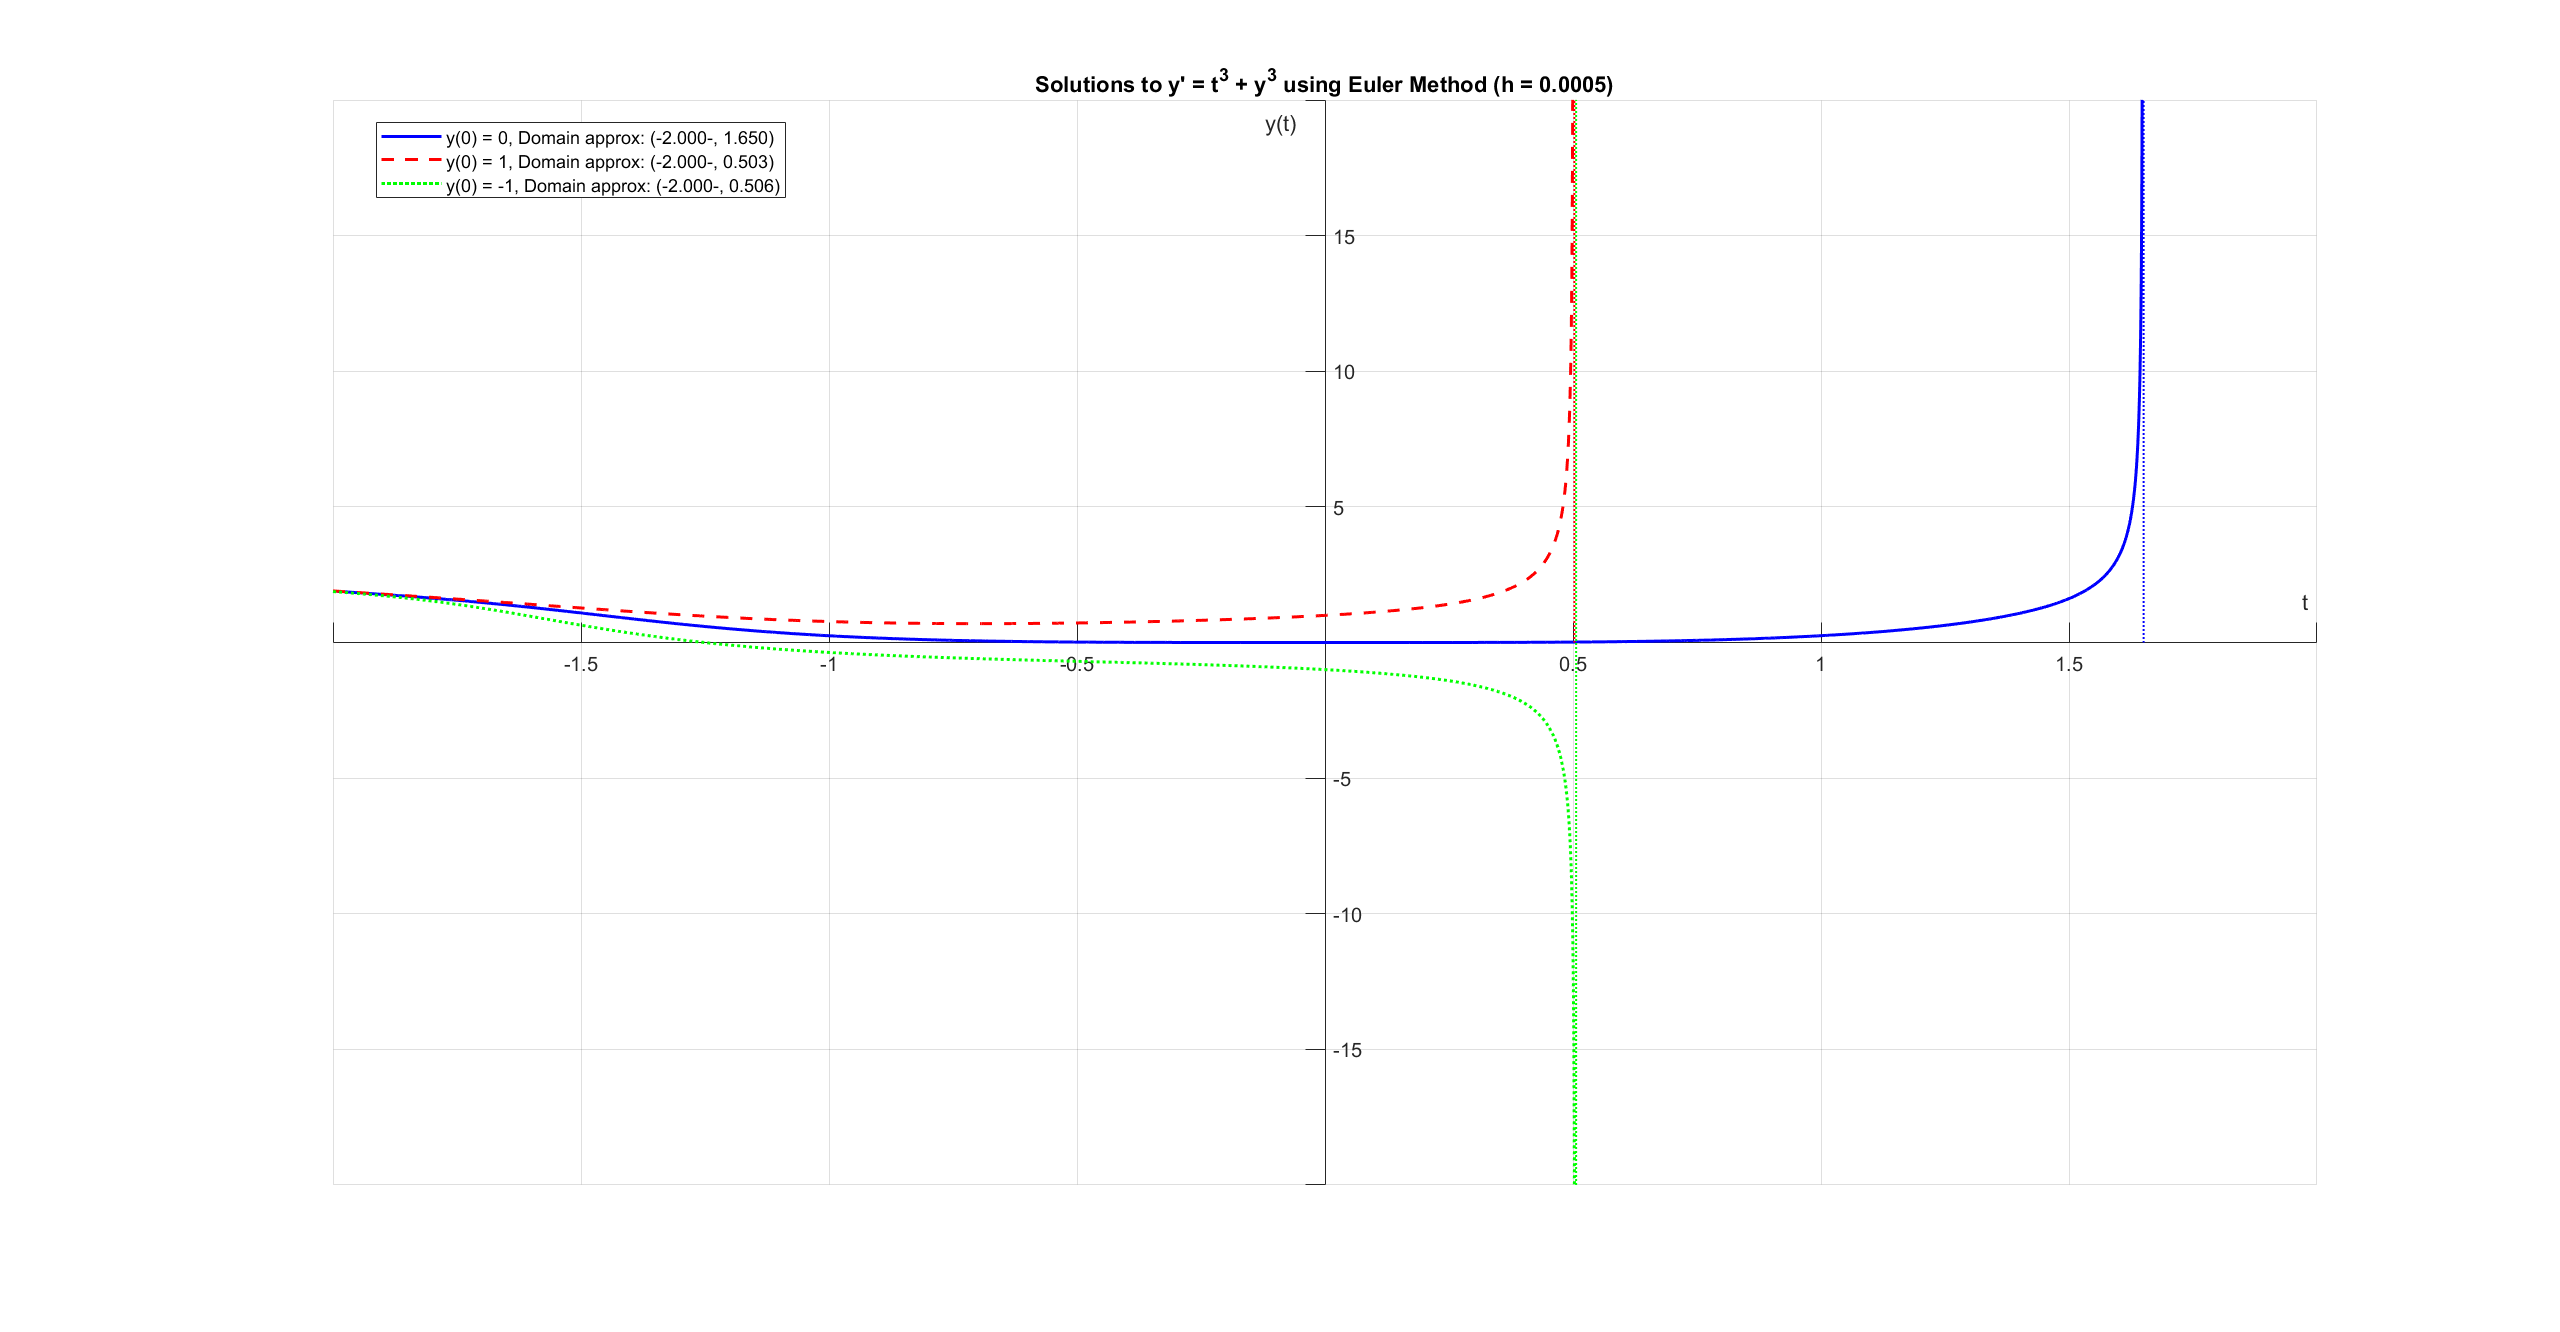
\includegraphics[width=0.7\textwidth]{pic/euler1.png}
    \caption{Euler Method}
    \label{fig: Euler Method}
\end{figure}

\subsubsection{Error Analysis}
A smaller step size $h$ generally leads to a more accurate approximation of the solution, but requires more computational steps. The local truncation error (error in one step) for the Euler method is $O(h^2)$, and the global truncation error (total accumulated error) is $O(h)$.

$y_0$ = 1 :
\begin{figure}[htbp]
    \centering
    \begin{minipage}[b]{0.45\textwidth}
        \centering
        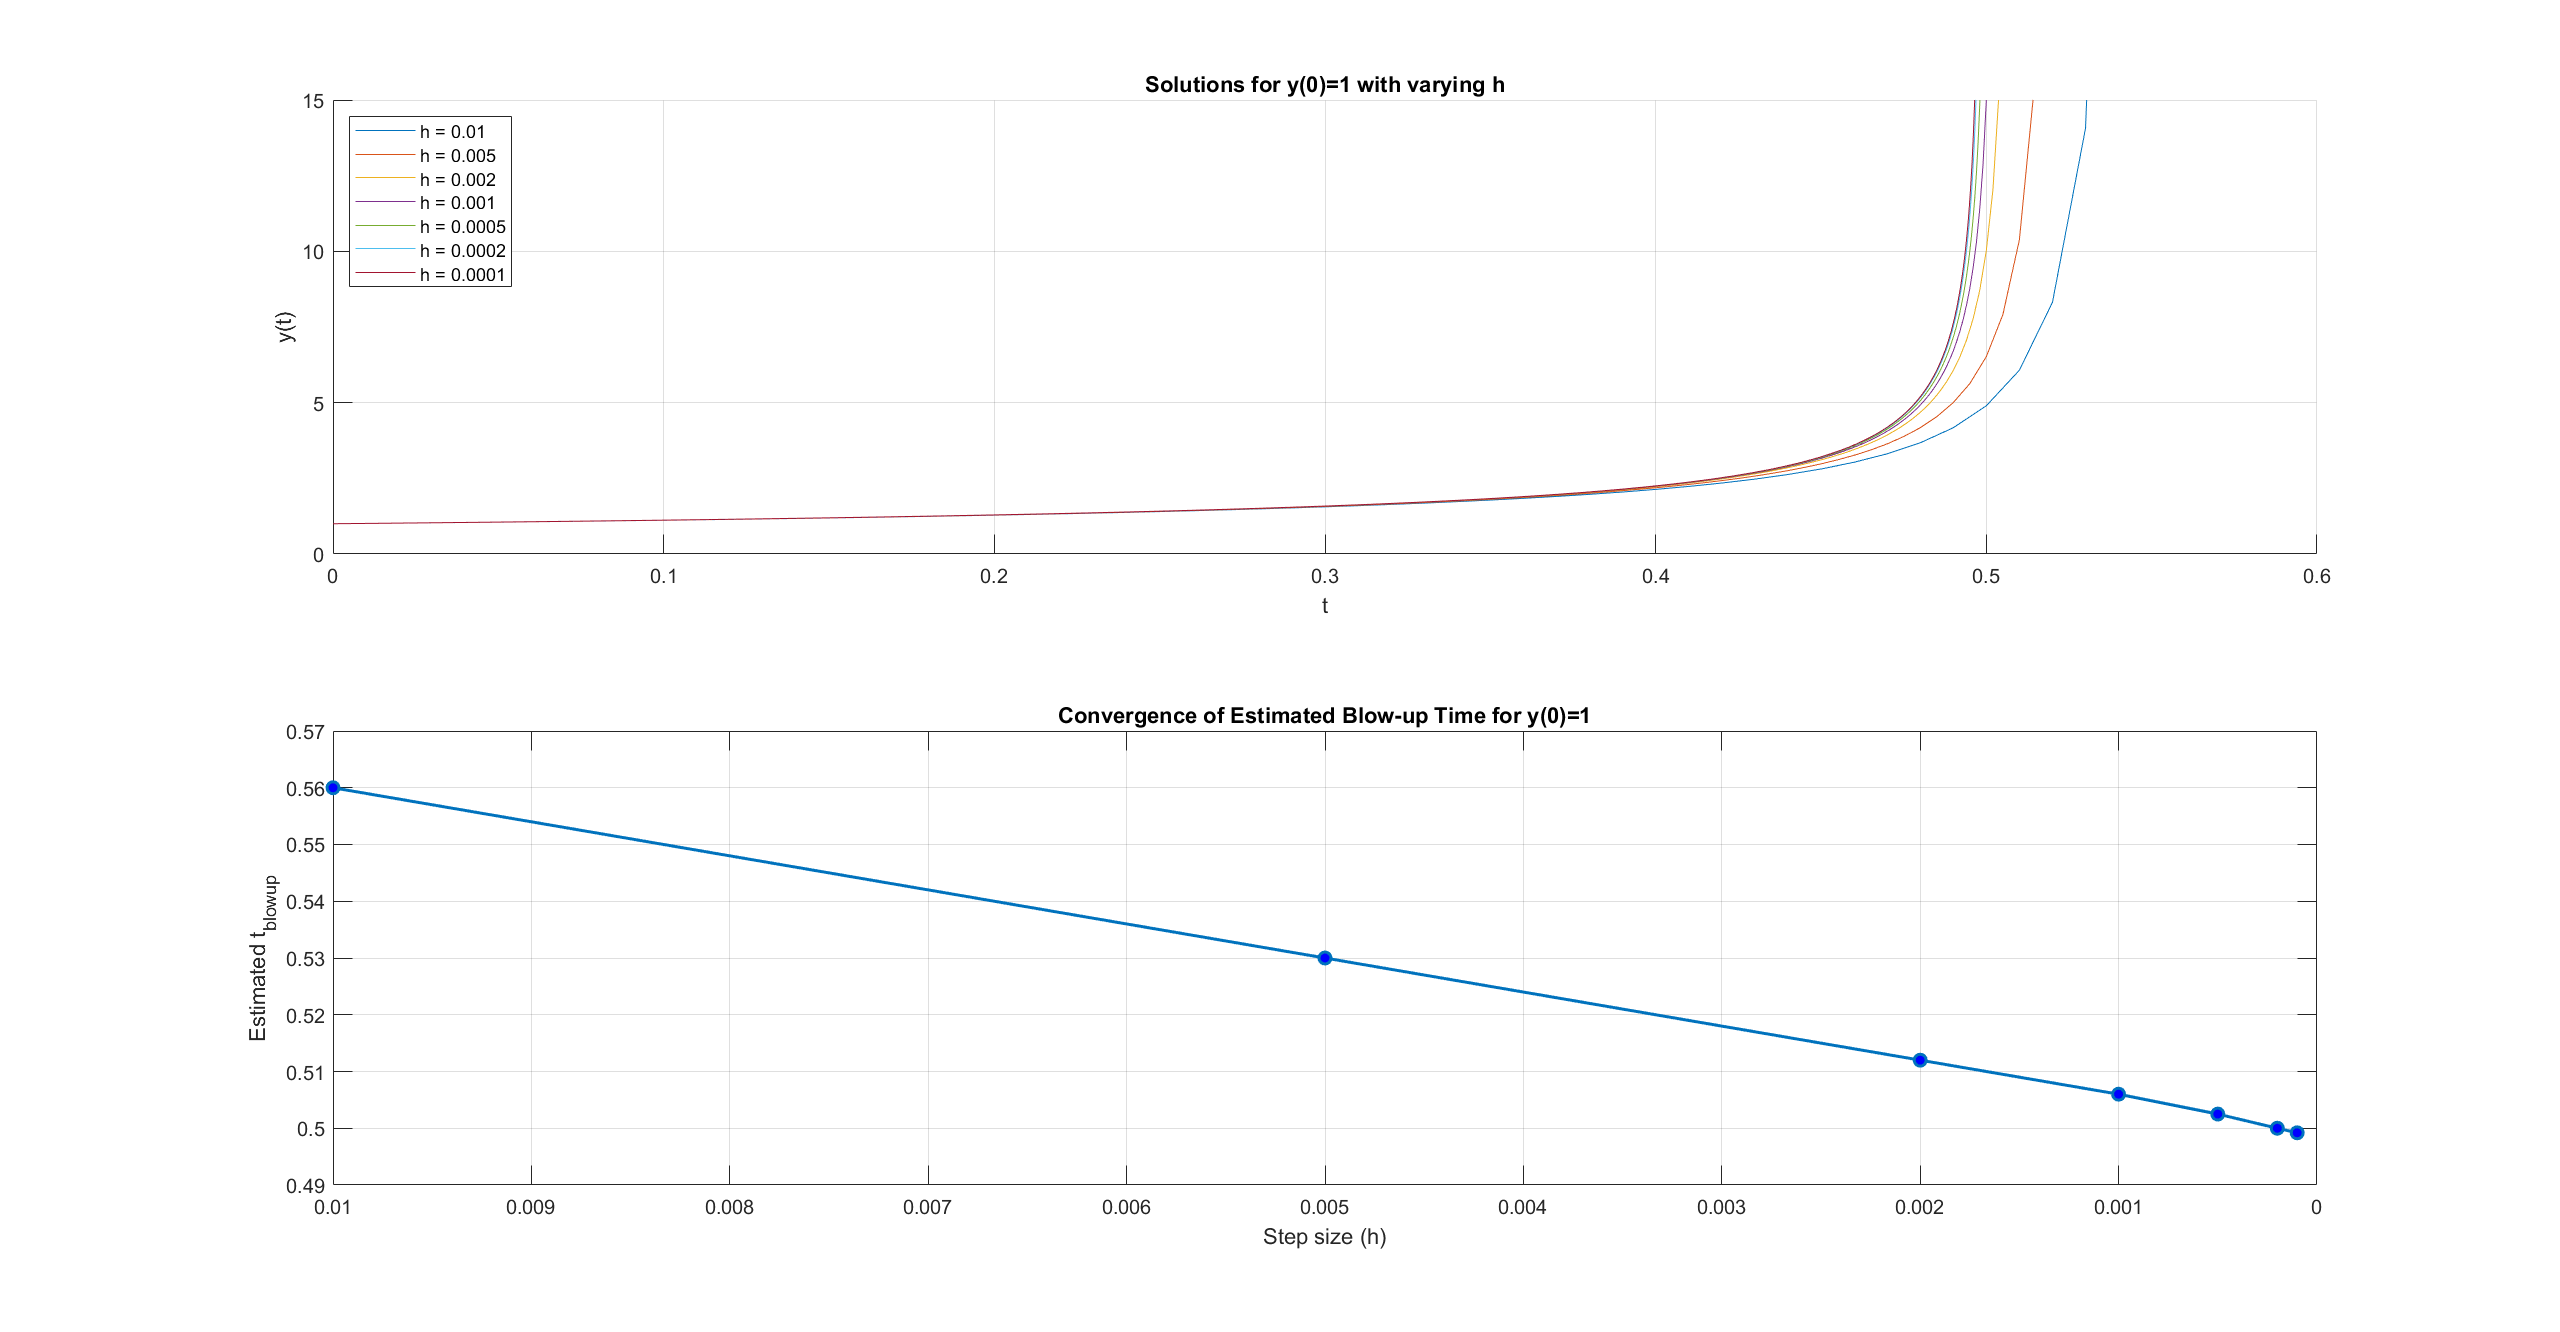
\includegraphics[width=\textwidth]{pic/euler_err1-1.png }
        \caption{Estimated $t_{blowup}$ vs. $h$}
        \label{fig:image1}
    \end{minipage}
    \hspace{0.05\textwidth}
    \begin{minipage}[b]{0.45\textwidth}
        \centering
        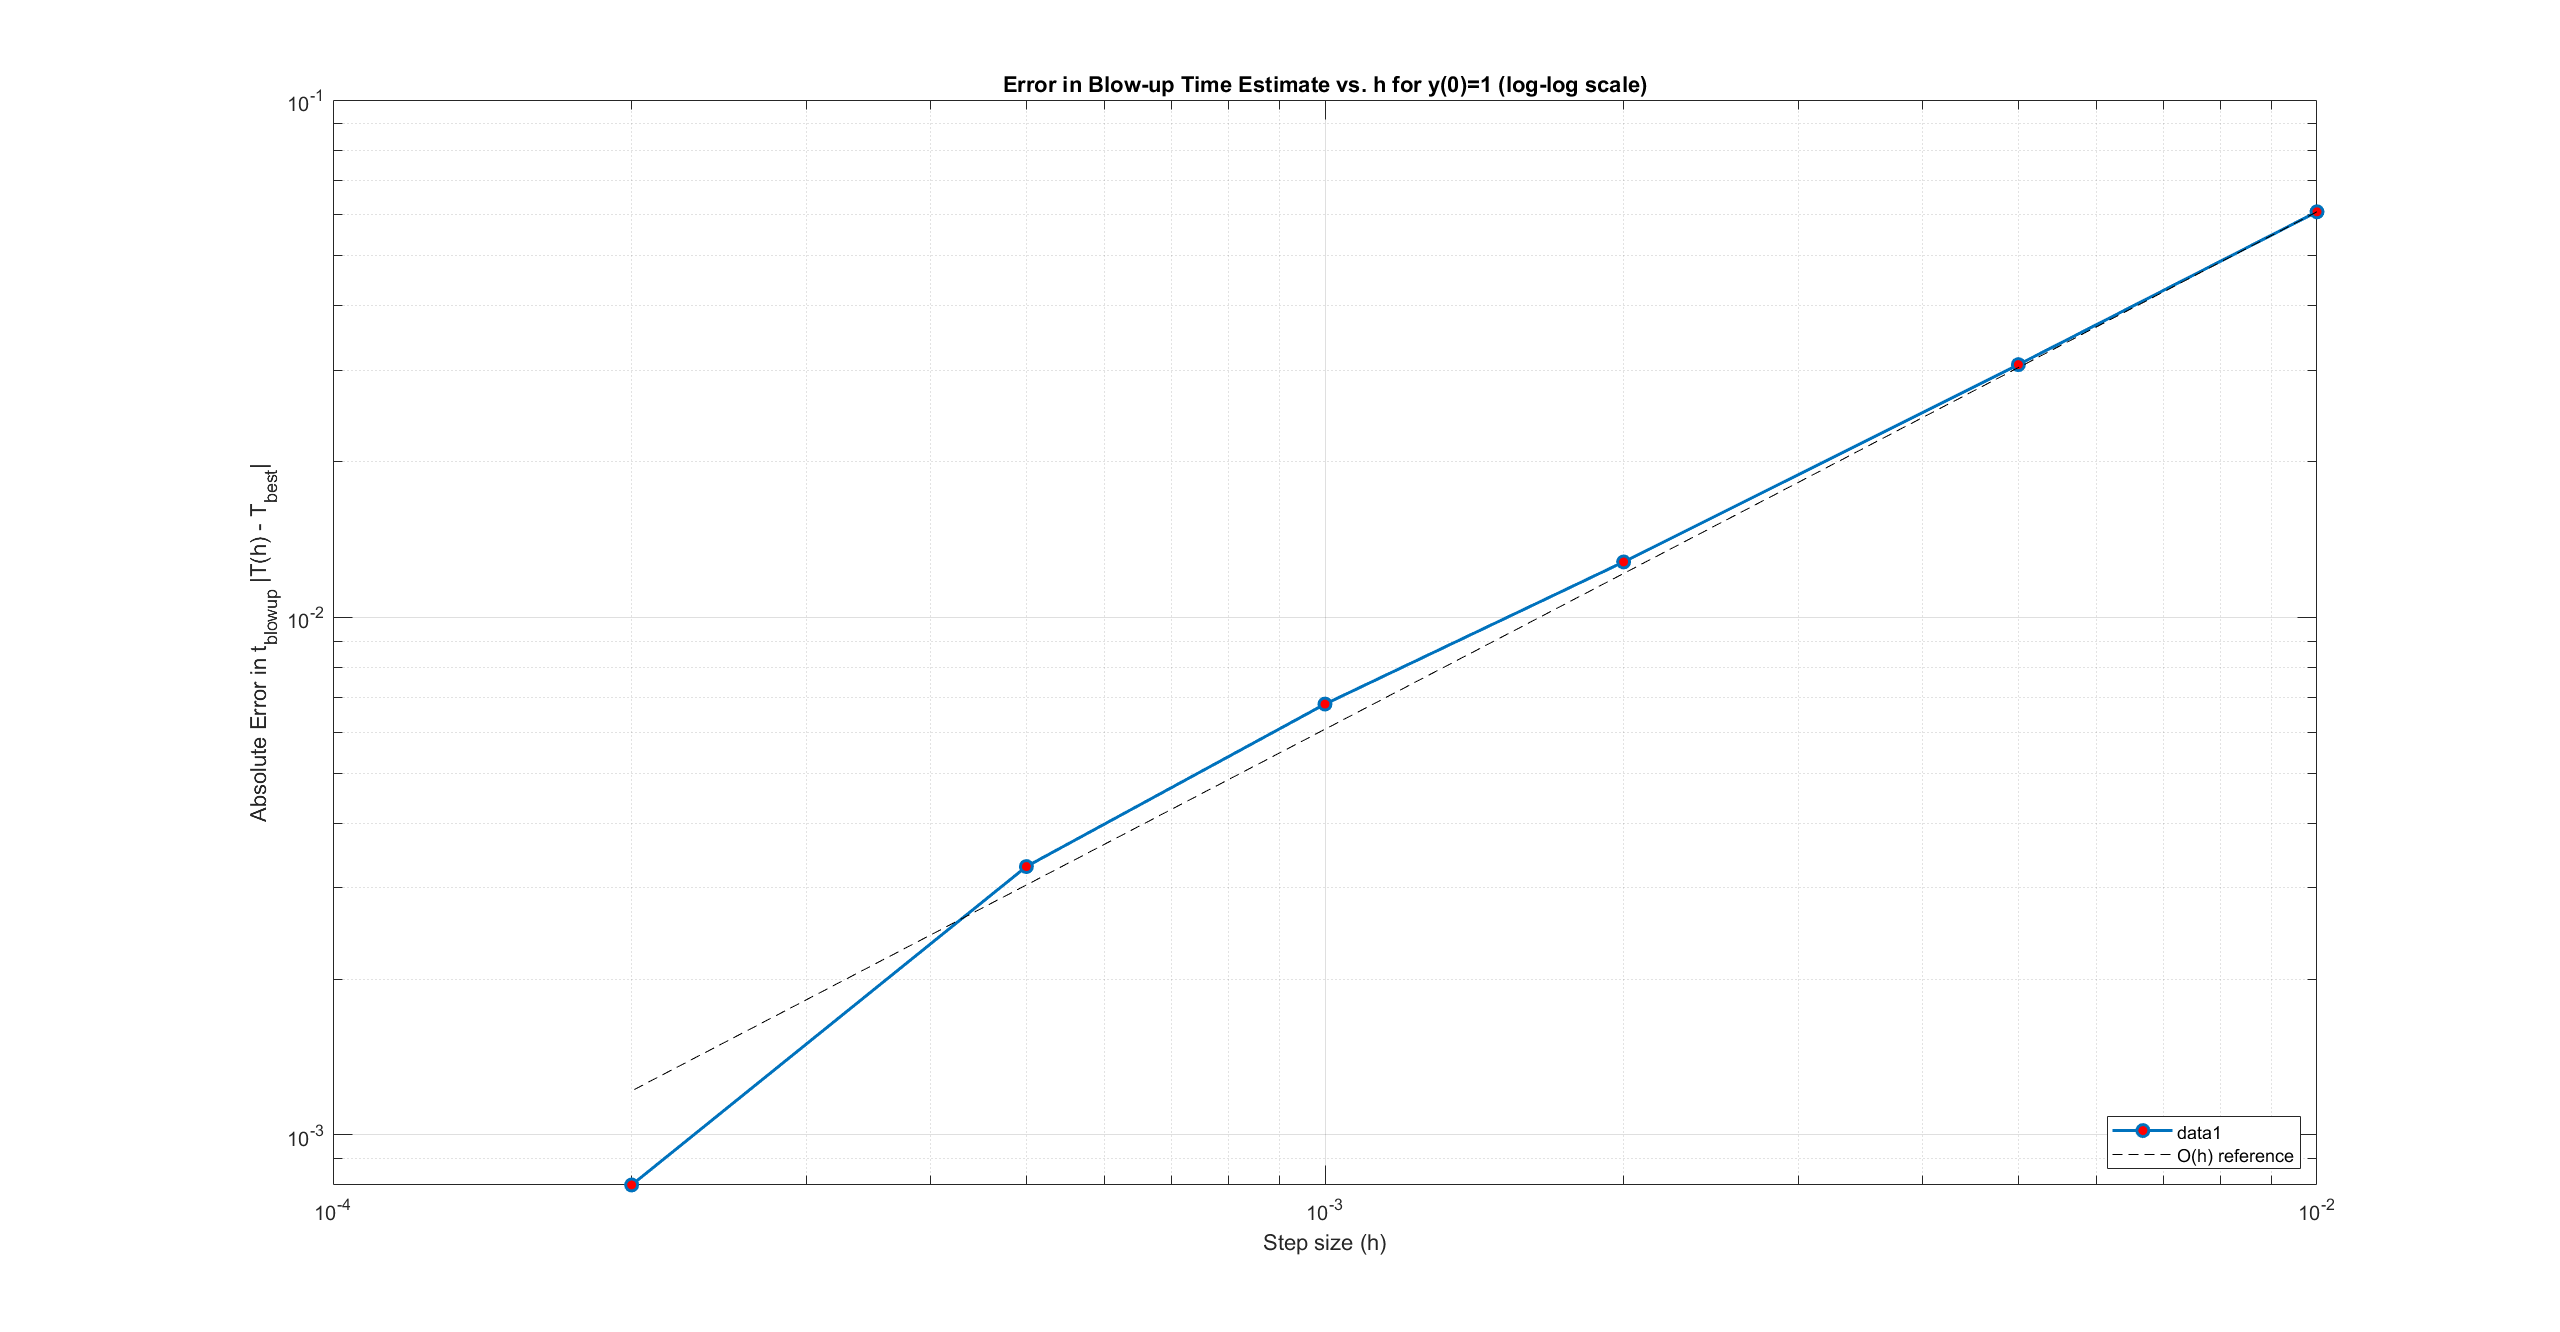
\includegraphics[width=\textwidth]{pic/euler_err1-2.png}
        \caption{Error in $t_{blowup}$ vs. $h$ (Log-Log Scale) }
        \label{fig:image2}
    \end{minipage}
\end{figure}




$y_0$ = -1 :
\begin{figure}[htbp]
    \centering
    \begin{minipage}[b]{0.45\textwidth}
        \centering
        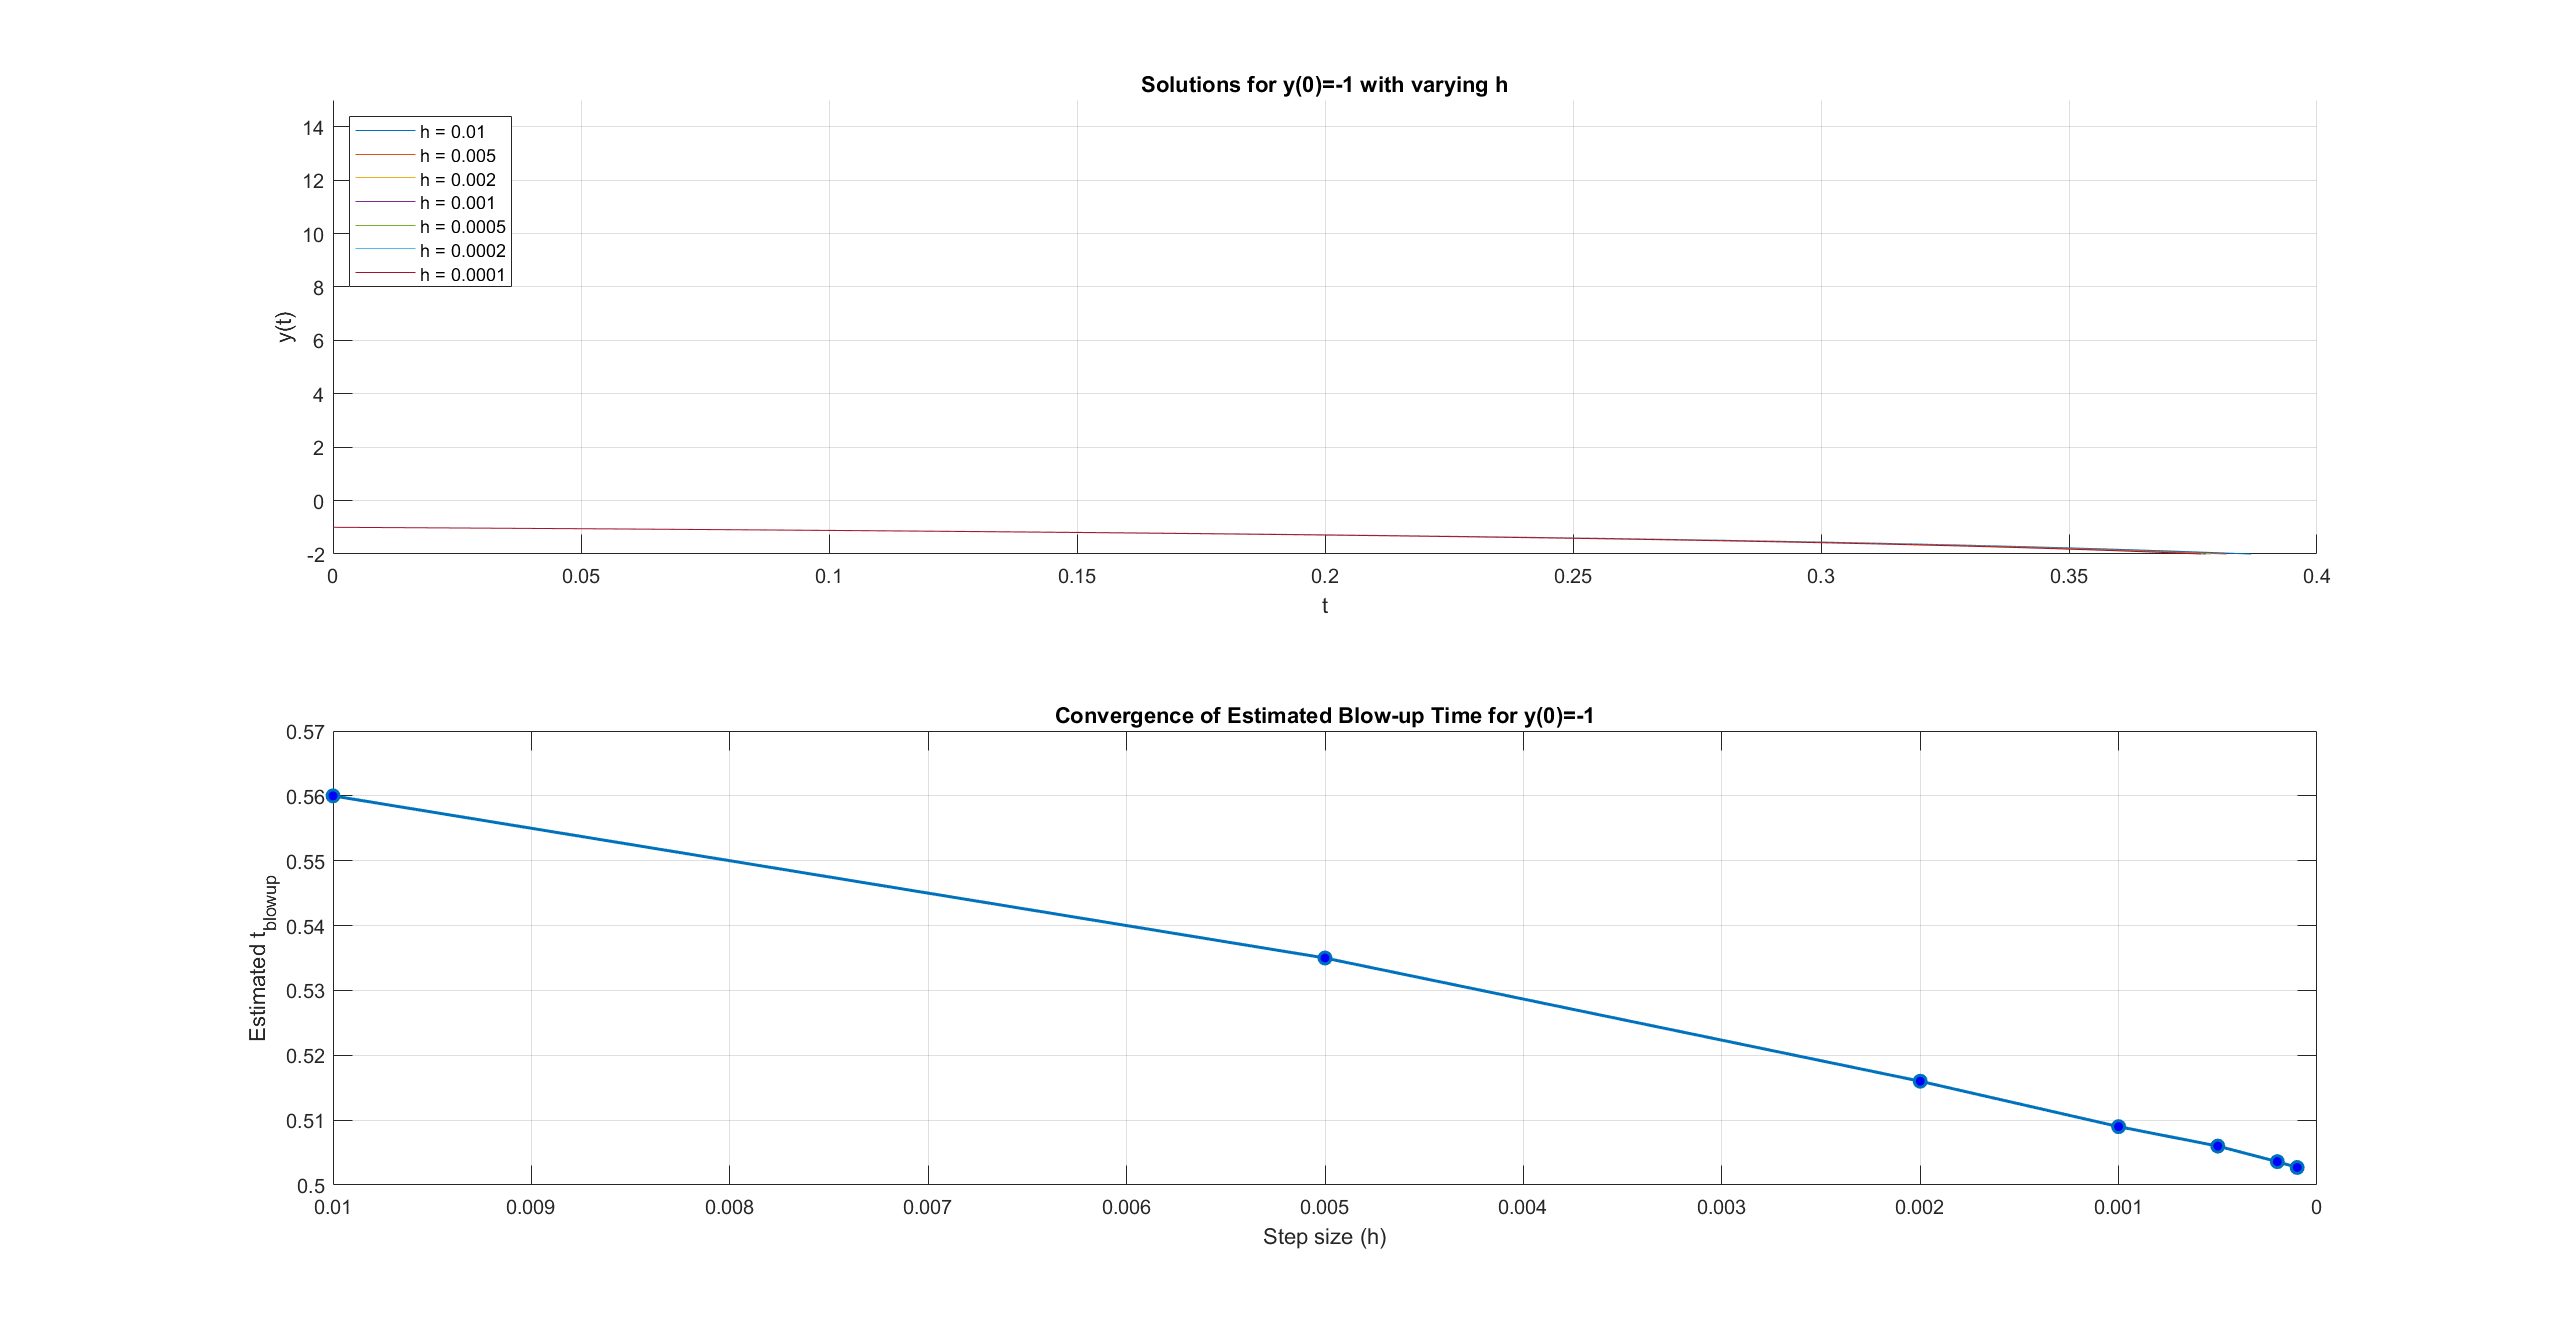
\includegraphics[width=\textwidth]{pic/euler_err-1-1.png }
        \caption{Estimated $t_{blowup}$ vs. $h$}
        \label{fig:image1}
    \end{minipage}
    \hspace{0.05\textwidth}
    \begin{minipage}[b]{0.45\textwidth}
        \centering
        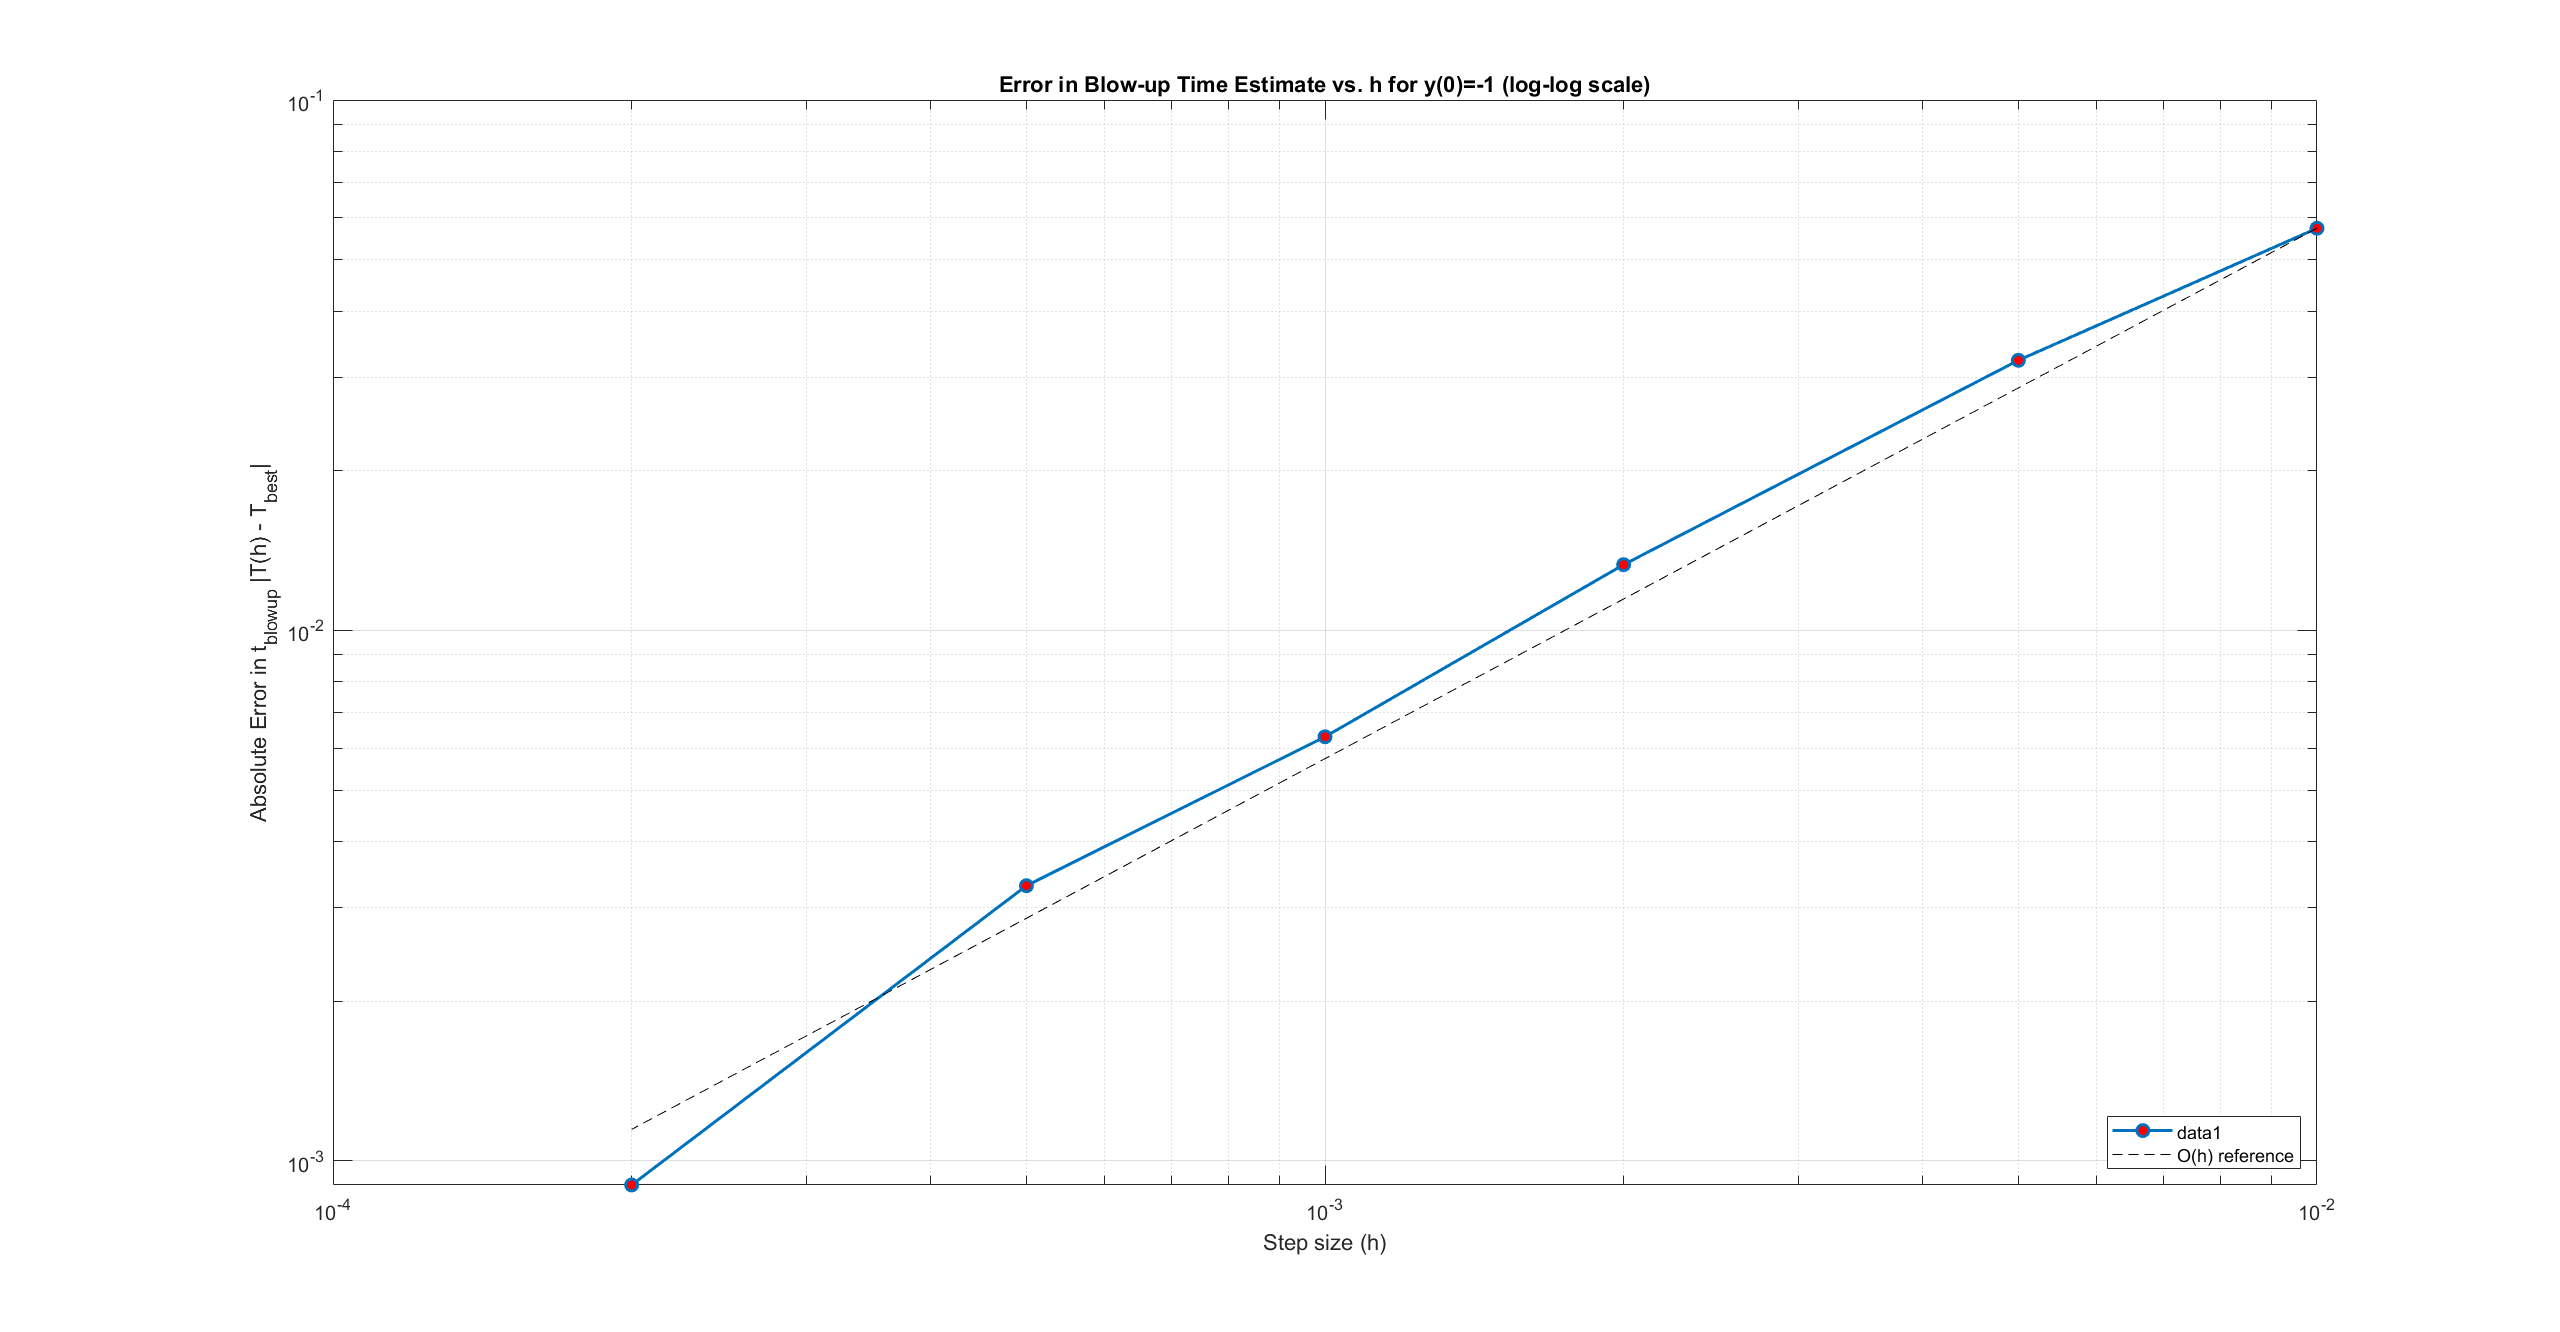
\includegraphics[width=\textwidth]{pic/euler_err-1-2.png}
        \caption{Error in $t_{blowup}$ vs. $h$ (Log-Log Scale) }
        \label{fig:image2}
    \end{minipage}
\end{figure}

\paragraph{$y_0$ = 0} : 
\begin{figure}[htbp]
    \centering
    \begin{minipage}[b]{0.45\textwidth}
        \centering
        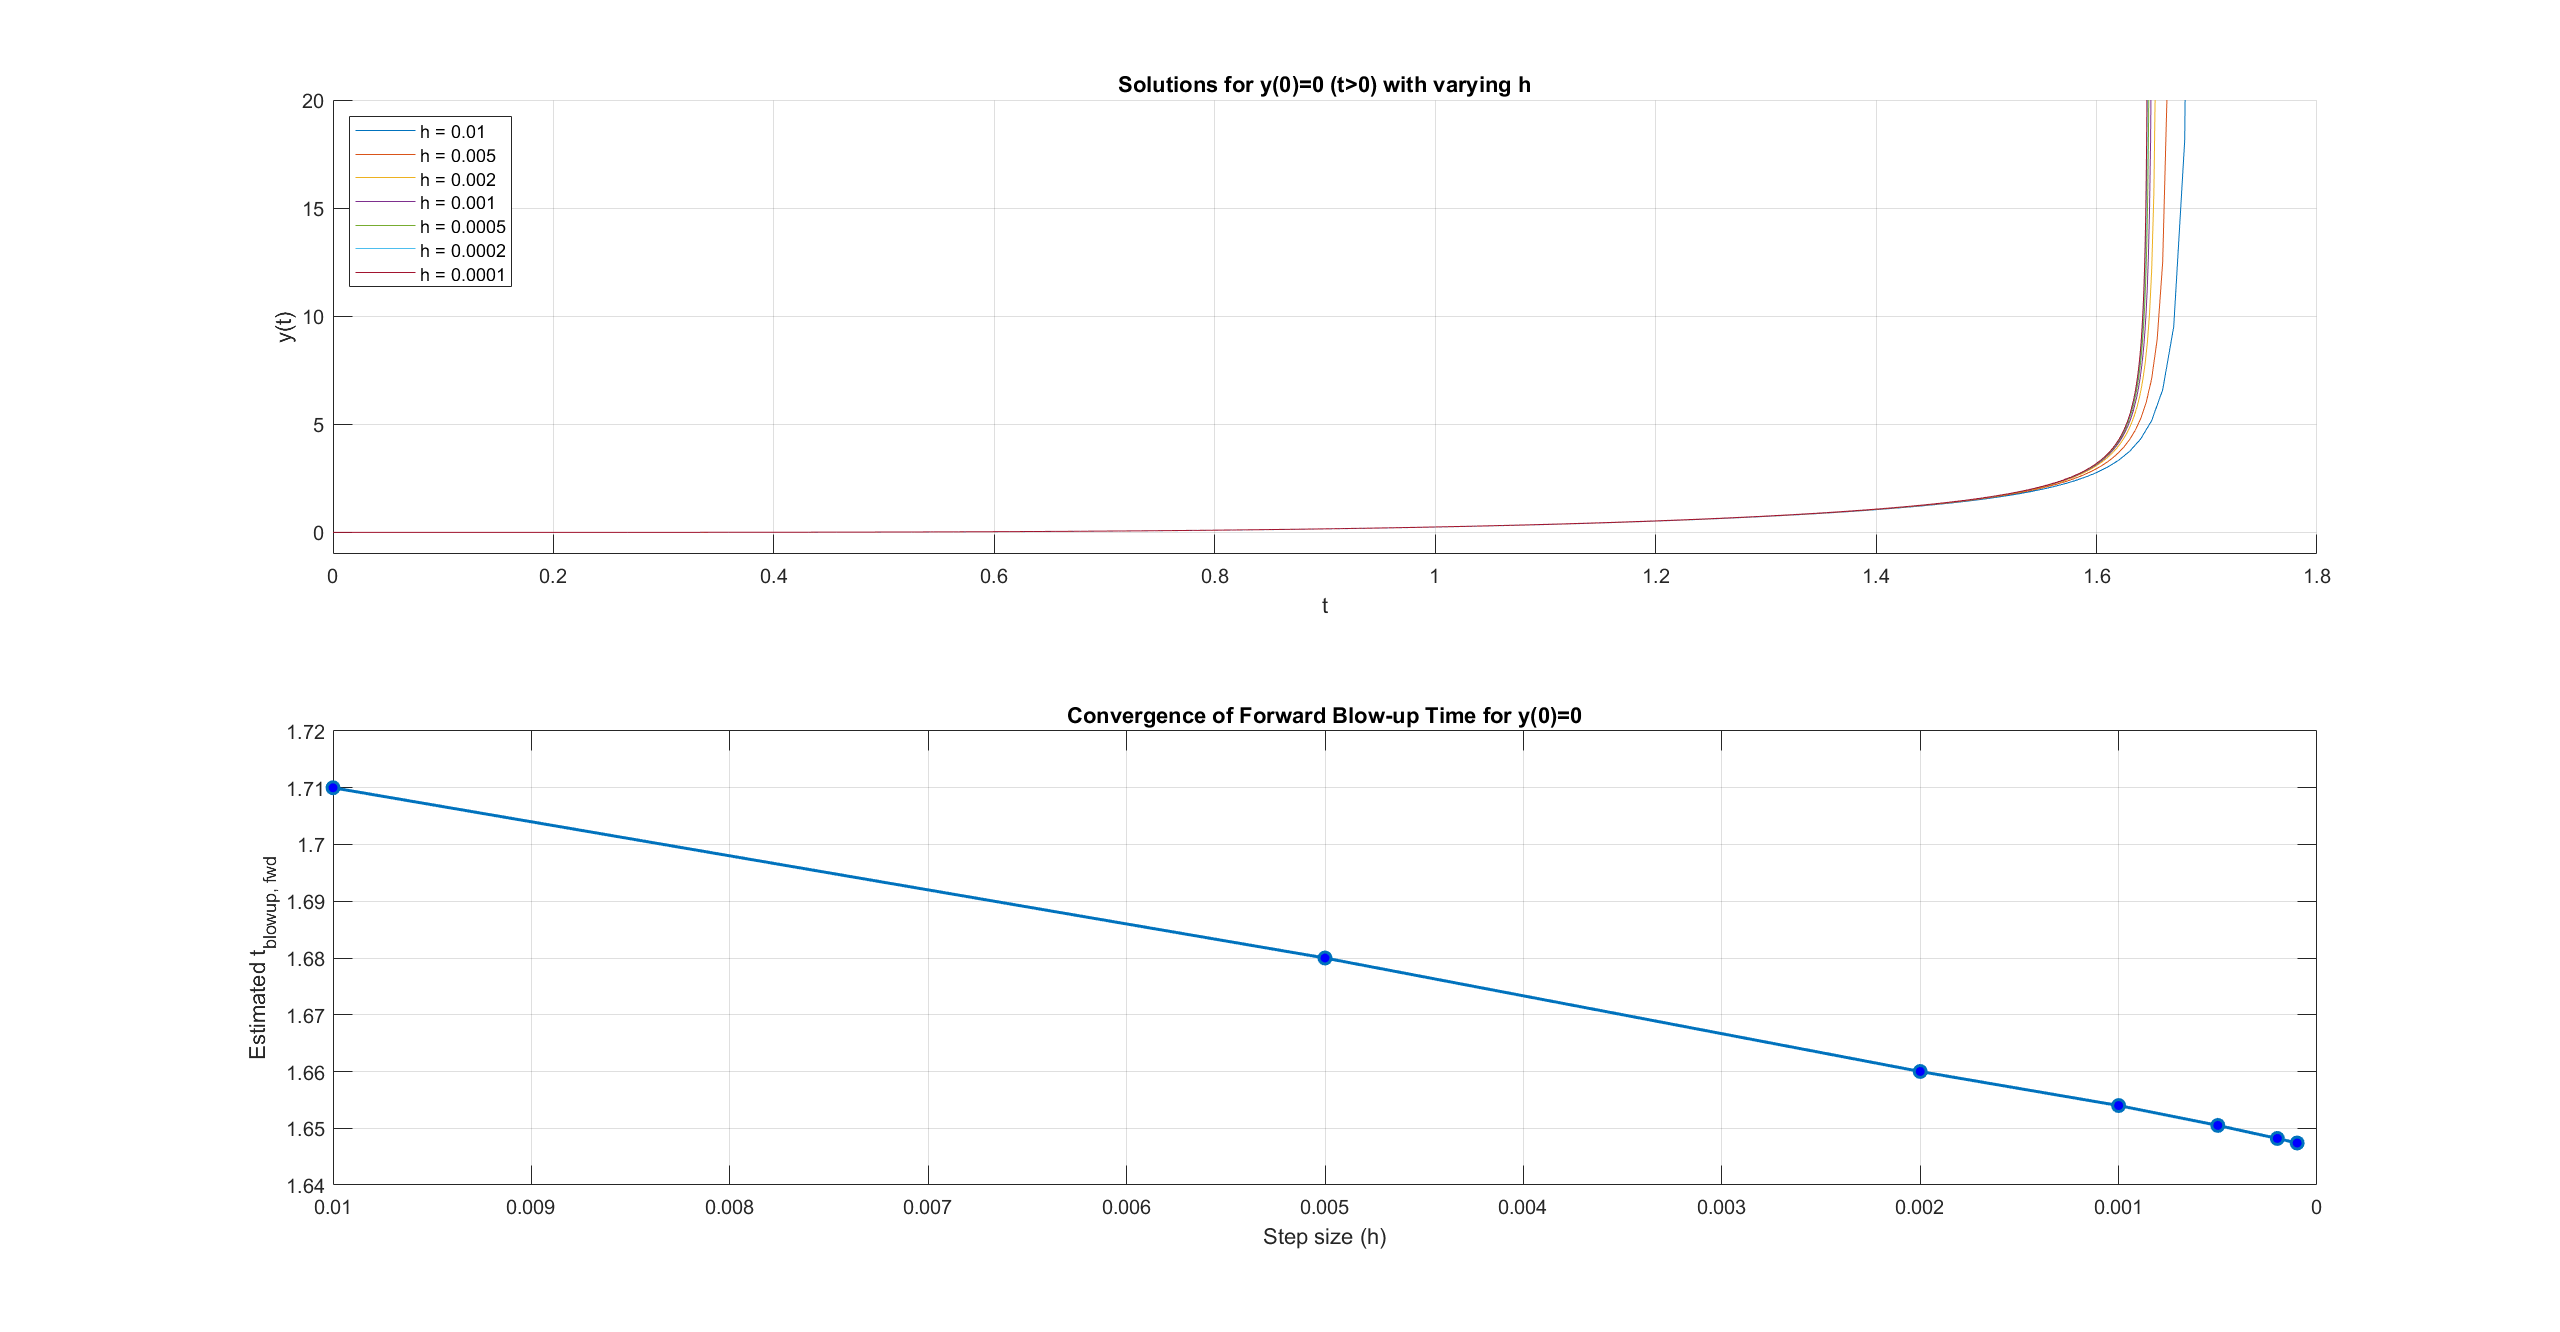
\includegraphics[width=\textwidth]{pic/euler_err0-1.png }
        \caption{Estimated $t_{blowup}$ vs. $h$}
        \label{fig:image1}
    \end{minipage}
    \hspace{0.05\textwidth}
    \begin{minipage}[b]{0.45\textwidth}
        \centering
        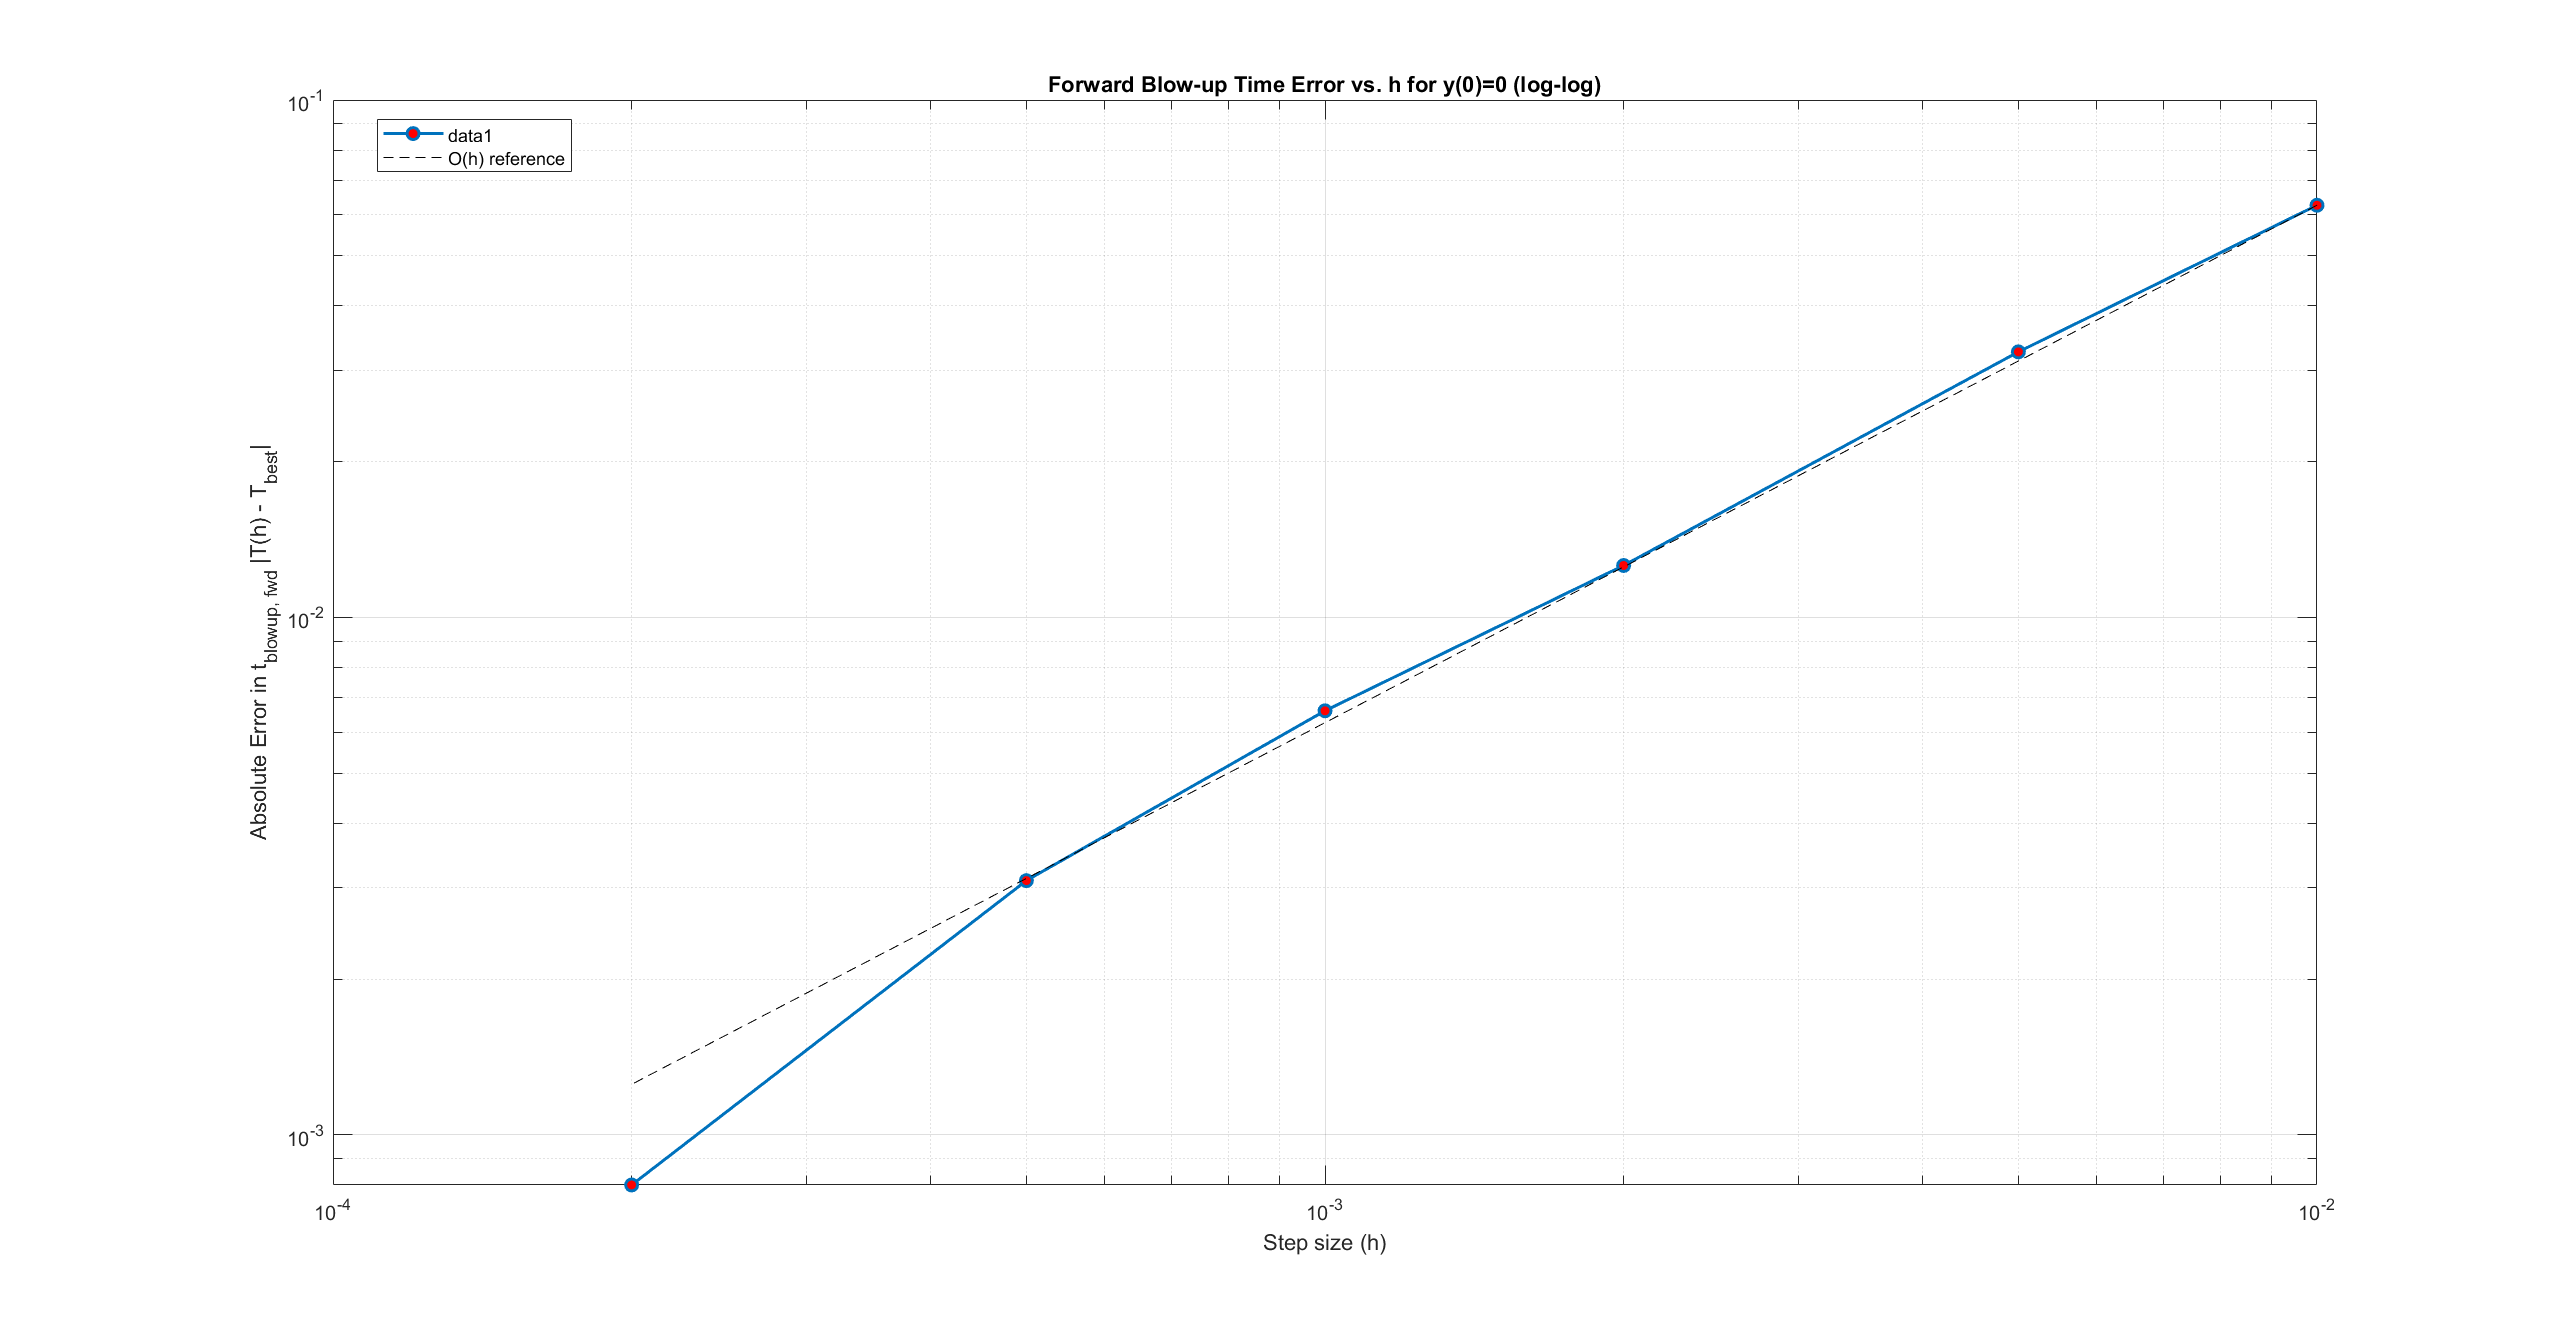
\includegraphics[width=\textwidth]{pic/euler_err0-2.png}
        \caption{Error in $t_{blowup}$ vs. $h$ (Log-Log Scale) }
        \label{fig:image2}
    \end{minipage}
\end{figure}


%%%%%%%%%%%%%%%%%%%%%%%%%%%%%%%%%%%%%%%%%%%%%%%%%%%%%%%%%%%%%%%%%%%%%%%
\subsection{Improved Euler Method}

\subsubsection{Mathematical Analysis}
The improved Euler method (also known as the Heun method or trapezoidal method) enhances accuracy by incorporating the trapezoidal integration formula. The basic idea is to use the average slope between the current point and the predicted point to estimate the next point's value. For a given ODE \( y' = f(t, y) \) with initial condition \( y(t_0) = y_0 \), the improved Euler method's recurrence formula is:
\[
y_{n+1} = y_n + \frac{h}{2} \left[ f(t_n, y_n) + f(t_{n+1}, y_{n+1}^{\text{predict}}) \right]
\]
where:
\begin{itemize}
    \item \( y_{n+1}^{\text{predict}} = y_n + h f(t_n, y_n) \) is the Euler method prediction.
\end{itemize}

The improved Euler method can be viewed as applying the trapezoidal rule to the integration problem. By considering the average slope at two adjacent points, the local truncation error is \( O(h^3) \), and the global truncation error is \( O(h^2) \).

\subsubsection{Result Presentation}

\begin{figure}[htbp]
    \centering
    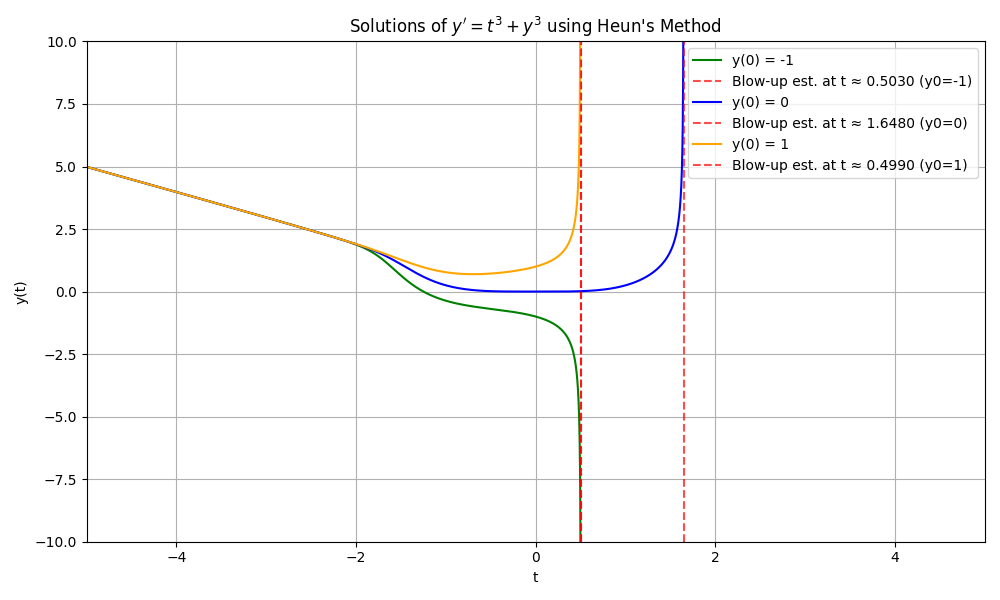
\includegraphics[width=0.8\textwidth]{pic/Figure_1.png}
    \caption{Improved Euler Method}
    \label{fig:Improved Euler Method}
\end{figure}

\subsubsection{Error Analysis}

The improved Euler method is a second-order method with a local truncation error of \( O(h^3) \) and a global truncation error of \( O(h^2) \). Compared to the Euler method, the improved Euler method is more stable when dealing with nonlinear and stiff problems. In this study, the improved Euler method shows higher accuracy and stability at the same step size, better capturing the solution's behavior.

% \subsubsection*{2.5.3 Error Analysis}

For \textbf{IVP1} (\( y' = t^3 + y^3, \ y(0) = -1 \)), the solution curve is relatively flat and stable, with no explosive behavior in the visualized domain. The improved Euler method provides a smooth, gradually increasing curve that closely follows the expected trend, indicating accurate approximation in this region.

For \textbf{IVP2} (\( y' = t^3 + y^3, \ y(0) = 0 \)), the solution remains regular but begins to exhibit accelerated growth as \( t \) increases. The improved Euler method remains stable under moderate step sizes, though minor divergence from the expected curve begins to appear as \( y^3 \) dominates.

For \textbf{IVP3} (\( y' = t^3 + y^3, \ y(0) = 1 \)), the solution exhibits rapid blow-up behavior. The improved Euler method is still able to track the solution before the blow-up time, though numerical instability may eventually occur if the step size is not sufficiently small. Compared to the standard Euler method, this approach offers improved robustness even in stiff or rapidly growing regimes.


\subsubsection{Conclusion}

Compared to the classical Euler method, the improved Euler method provides higher accuracy and better stability when applied to the nonlinear equation \( y' = t^3 + y^3 \) under different initial conditions. It is especially advantageous in handling rapidly changing or stiff-like behavior such as in IVP3.

The comparative analysis of IVP1--IVP3 demonstrates that the improved Euler method performs well across all three scenarios, particularly by suppressing error growth in IVP2 and better tracking pre-blow-up behavior in IVP3. This confirms its effectiveness in approximating solutions to nonlinear problems.

While the improved Euler method requires slightly more computation per step than the Euler method, its overall benefits in accuracy and stability make it a practical choice in solving ODEs with strong nonlinearities.

\subsection{Picard-Lindelof Iteration}

\subsubsection{Mathmatical Analysis}
Picard-Lindelof Iteration provides a way to approximate the initial value problem. In our problem, $f(t, y_n(t)) = t^3 + y_n^3(t) $, $y_0(t) = y(0)=y_0$
To ensure the applicability of the Picard-Lindelof iteration method, we need to check whether the function $f$ satisfies two key conditions within a rectangular region. 
\begin{itemize}
    \item Continuity of $f$: The function $f(t, y)$ is a polynomial function that means $f$ is continuous on $R^2$. 
    \item Lipschitz condition: If $y_1$ and $y_2$ are both in the interval $ [y_0 - b, y_0 + b] $, $|y|^2 \leq (|y_0|+b)^2$ for any $y \in  [y_0 - b, y_0 + b] $.  
    $$ | f (t, y_1) - f (t, y_2) | = (t3 + y_13) - (t3 + y_23) = y_13-y_23 = | (y_1-y_2) (y_12 + y_1 y_2 + y_2^2) |$$
    As $|(y_1^2 + y_1 y_2 + y_2^2) | \leq 3 (|y_0|+b)^2$, we can choose $L = 3 (|y_0|+b)^2 $. Then $|f(t, y_1) - f(t, y_2)| \leq L |y_1-y_2|$ is true in an rectangle region around $(t_0, y_0)$.
\end{itemize}
Then, we can use the Picard-Lindelof iteration to get an approximation of the IVP. 
$$ y_{n + 1}(t) = y_n(t) + \int_0^t f(s, y_n(s)) ds = y_n(t)+\int_0^t (s^3 + y_n^3(t))  ds$$

\subsubsection{Results Display}


\begin{itemize}
    \item $y_0=0$:
    \begin{align*}
        y_0(t) &= 0 \\
        y_1(t) &= y_0 + \int_0^t (s^3 + (y_0(s))^3) \, ds 
                = 0 + \int_0^t (s^3 + 0^3) \, ds 
                = \int_0^t s^3 \, ds 
                = \frac{t^4}{4} \\
        y_2(t) &= y_0 + \int_0^t (s^3 + (y_1(s))^3) \, ds 
                = 0 + \int_0^t \left( s^3 + \left( \frac{s^4}{4} \right)^3 \right) \, ds 
                = \int_0^t \left( s^3 + \frac{s^{12}}{64} \right) \, ds \\
        \ldots
    \end{align*}
\end{itemize}

\begin{figure}[htbp]
    \centering
    \begin{minipage}[b]{0.25\textwidth}
        \centering
        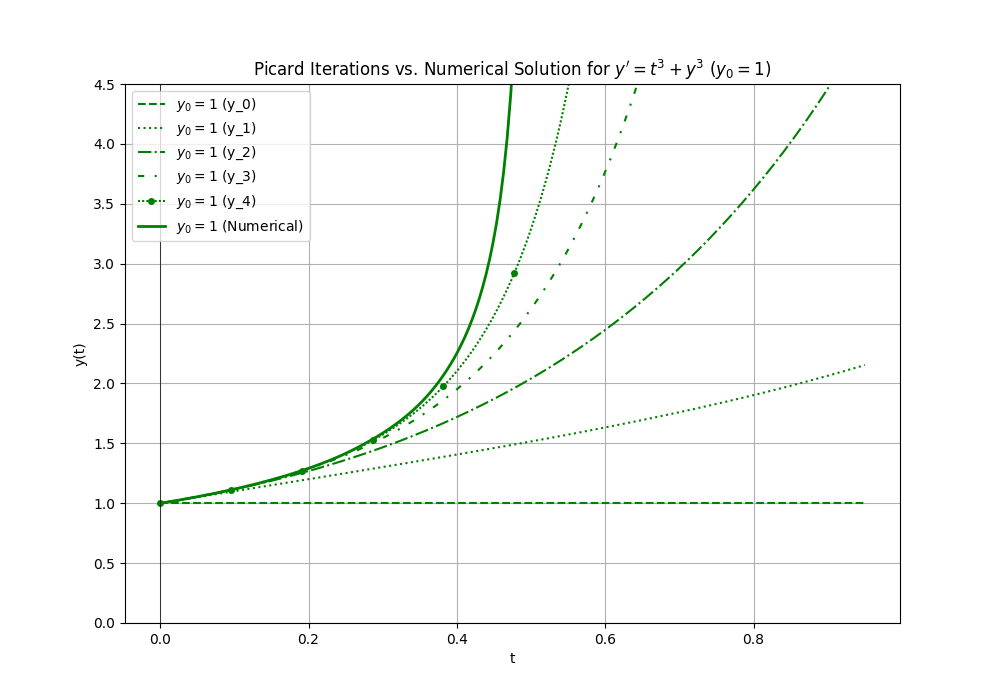
\includegraphics[width=\textwidth]{pic/Picard_1.png }
        \caption{Estimated $t_{blowup}$ vs. $h$}
        \label{fig:picard_1}
    \end{minipage}
    \hspace{0.05\textwidth}
    \begin{minipage}[b]{0.25\textwidth}
        \centering
        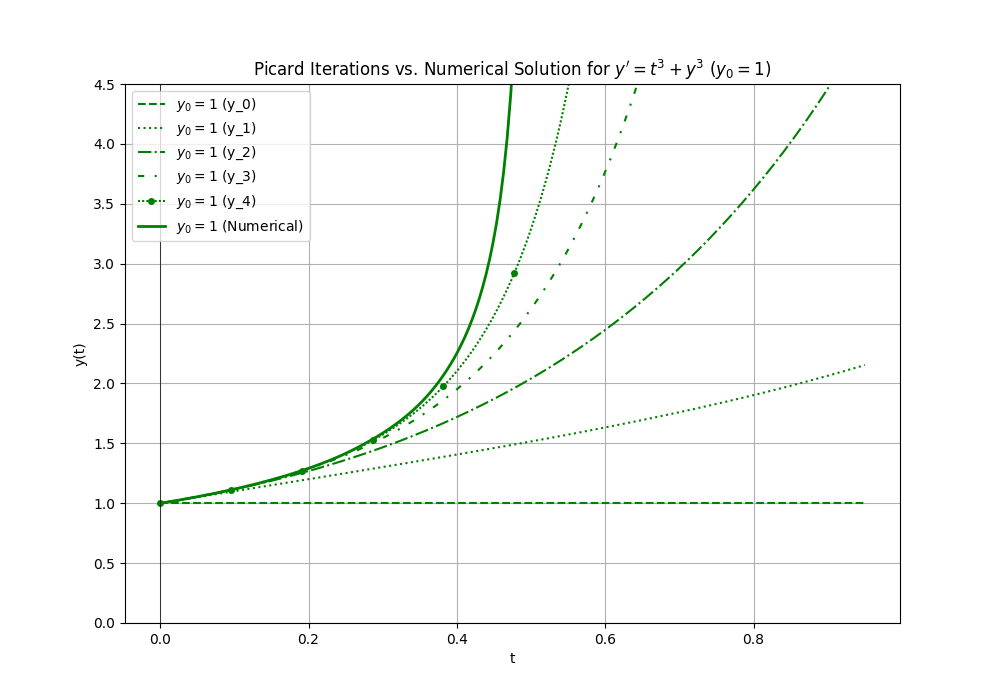
\includegraphics[width=\textwidth]{pic/Picard_1.png }
        \caption{Estimated $t_{blowup}$ vs. $h$}
        \label{fig:picard_1}
    \end{minipage}
    \hspace{0.05\textwidth}
    \begin{minipage}[b]{0.25\textwidth}
        \centering
        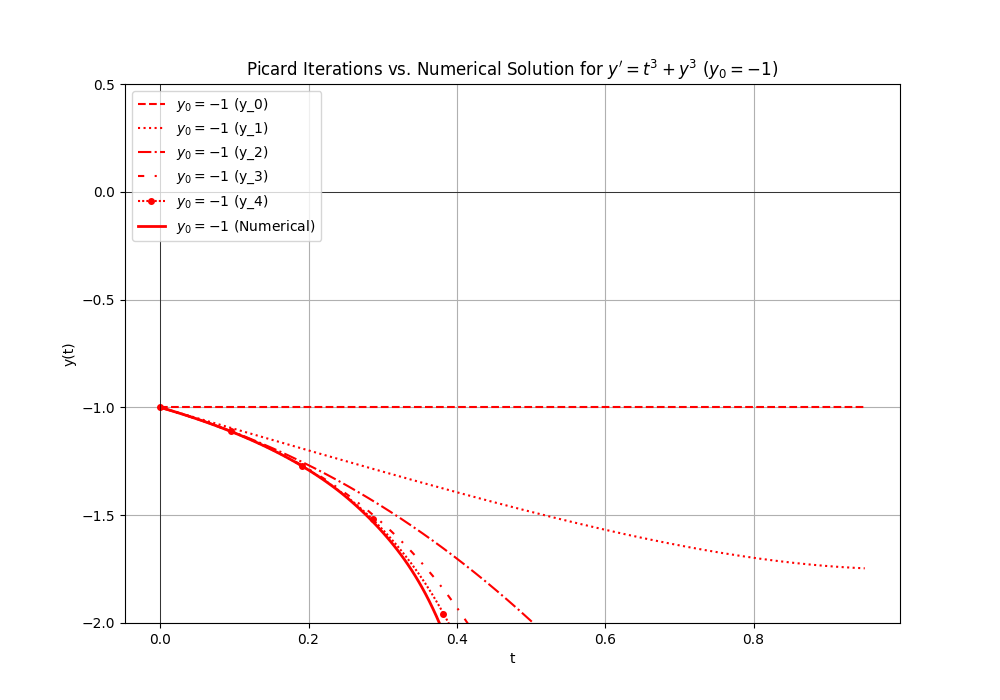
\includegraphics[width=\textwidth]{pic/Picard_-1.png}
        \caption{Error in $t_{blowup}$ vs. $h$ (Log-Log Scale) }
        \label{fig:picard_-1}
    \end{minipage}
\end{figure}

\subsubsection{Error Analysis}
Picard-Lindelof theorem provides an error bound for $n$-th iterate $y_n(t)$. 
$$y(t)-y_n(t) \leq \frac{ML^n |t-t_0|^{n+1}}{(n+1)!}$$
Where $M=\textbf{max}|f(t,y)|$ in region $R=[t_0-a, t_0 +a] \times [y_0-b, y_0+b]$, $L$ is the constant in Lipschitz condition. In our situation, $M = a^3 + (y_0+b)^3$, $L = 3(|y0|+b)^2$. Since the factorial function grows faster than the exponential function, the limit tends to zero. 



\subsection{Series method}

\subsubsection{Method}
    The series method is to use a power series as the analytic solution.
    \[
        y(t) = \sum_{n=0}^{\infty} a_n (t - t_0)^n, \quad t \in I
    \]
    Basically, there are two methods to obtain the best series. In first method, the solution will be obtained by the following steps.
\\ \\
\textbf{First Method :}
\begin{itemize}
\item  \text{Determine the $n^{\text{th}}$ derivative of the given ODE.}
\begin{align*}
y^{(1)} &= t^3 + y^3 \\
y^{(2)} &= 3t^2 + 3y^2 \cdot y^{(1)}=3t^2 + 3 y^5 + 3y^2t^3 \\ 
y^{(3)} &= 6t + 3 y^2 \cdot y^{(2)} + 6y \cdot y^{(1)^2} \\
y^{(4)} &= 6 + 6y \cdot y^{(2)} +3 y^2 \cdot y^{(3)} + 6 y^{(1)^2} + 12y \cdot y^{(1)} \cdot y^{(2)}
\end{align*}
\end{itemize}


\begin{itemize}
    \item Get the value using initial values.
\begin{align*}
\textbf{while } & y(0) = -1,y^{(1)}(0) = -1,y^{(2)}(0) = -3,y^{(3)}(0) = -15 \\
\textbf{while } & y(0) = 0,y^{(1)}(0) = 0,y^{(2)}(0) = 0,y^{(3)}(0) = 0,y^{(4)}(0) = 6 \\
\textbf{while } & y(0) = 1,y^{(1)}(0) = 1,y^{(2)}(0) = 3,y^{(3)}(0) = 15 \\
\end{align*}
\end{itemize}

\begin{itemize}
    \item Compute the solution
\begin{align*}
    \textbf{While } y(0) &= -1,y(t) = -1 + \frac{-1}{1!}t + \frac{-3}{2!} t^2 + \frac{-15}{3!} t^3 + \cdots \\
    \textbf{While } y(0) &= 0,
    y(t) = 0 + \frac{0}{1!}t + \frac{0}{2!} t^2 + \frac{0}{3!} t^3 + \frac{6}{4!} t^4 + 
   \cdots \\
    & \textbf{(In this case, the solution start from 4th number) }
\\
    \textbf{While } y(0) &= 1,
    y(t) = 1 + \frac{1}{1!}t + \frac{3}{2!} t^2 + \frac{15}{3!} t^3 + \cdots \\
\end{align*}
\end{itemize}

Then, we can compute the similar result by using the second method. \\ \\
\textbf{Second Method :}
\begin{itemize}
    \item As the given function, we could obtain the first derivative.
    \begin{align*}
        y(t) &= \sum_{n=0}^{\infty} a_n \cdot t^n,
        y^{(1)}(t) = n\cdot \sum_{n=0}^{\infty} a_n \cdot t^{n-1}
    \end{align*}
\end{itemize}

\begin{itemize}
    \item According to ODE
    \begin{align*}
    & t^3 + y^3 =  y^{(1)} = \sum_{n=1}^{\infty} n\cdot a_n \cdot t^{n-1} 
         = \sum_{n=0}^{\infty} (n+1) \cdot a_{n+1} \cdot t^{n},y^3 = \left( \sum_{n=0}^\infty a_n t^n \right)^3 = \sum_{n=0}^\infty \left( \sum_{\substack{i+j+k = n \\ i,j,k \geq 0}} a_i a_j a_k \right) t^n \\
    & \text{So} \\
    & \sum_{n=0}^\infty \left( \sum_{\substack{i+j+k = n \\ i,j,k \geq 0}} a_i a_j a_k \right) t^n + t^{3} = \sum_{n=0}^{\infty} (n+1) \cdot a_{n+1} \cdot t^{n} \\
     \end{align*}
\end{itemize}

\begin{itemize}
    \item Calculate the coefficient
    \begin{align*}
        & \textbf{While } n \neq 3, (n+1) \cdot a_{n+1} = \sum_{\substack{i+j+k = n \\ i,j,k \geq 0}} a_i a_j a_k \\
        & \textbf{While } n=3,(n+1) \cdot a_{n+1} = \sum_{\substack{i+j+k = 3 \\ i,j,k \geq 0}} a_i a_j a_k +1 \\
    \end{align*}
\end{itemize}

\begin{itemize}
    \item Together with the initial value
    \begin{align*}
        \textbf{While } a_0 &= y(0) = -1,y(t) = -1 + \frac{-1}{1!}t + \frac{-3}{2!} t^2 + \frac{-15}{3!} t^3 + \cdots\\
        \textbf{While } a_0 &= y(0) = 0,y(t)  = 0 + \frac{0}{1!}t + \frac{0}{2!} t^2 + \frac{0}{3!} t^3 + \frac{6}{4!} t^4 + 
   \cdots\\
        \textbf{While } a_0 &= y(0) = 1,y(t)  = 1 + \frac{1}{1!}t + \frac{3}{2!} t^2 + \frac{15}{3!} t^3 + \cdots \\
    & \textbf{All solutions are the same as previous methods}
    \end{align*}

    
\end{itemize}

\subsubsection{Results Display}

By using computer program, we can show the the third IVP in the following series function.
\begin{align*}
    y(t) = 1 + t + \frac{3}{2} t^2 + \frac{5}{2}t^3 + \frac{37}{8} t^4 + \frac{321}{40}t^5 + \frac{197}{40} t^6 + \frac{713}{280} t^7 + \frac{289}{224} t^8 + \frac{2939}{2880}t^9 + \cdots
\end{align*}

\subsubsection{Error Analysis}
The result seems fit well in positive part. We noticed that there are some difference in the figure (below) but that is because we only use first ten items to draw this figure, if we use first fifty, the answer will be better.
    
    \begin{figure}[htbp]
    \centering
        \centering
        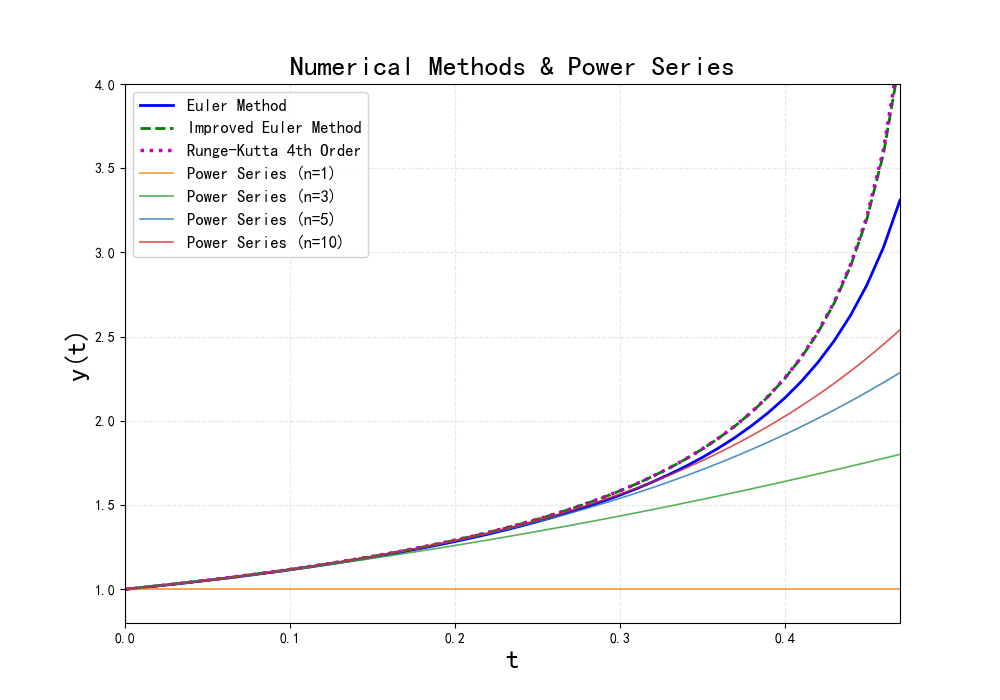
\includegraphics[width=0.6\textwidth]{pic/series.png }
        \caption{Series Solution of IVP with $y(0)=1$}
        \label{fig:Picard_-1}
    \end{figure}

We can also see that as the number of item increase the solution is more accurate.
\subsection{Runge-Kutta method}




\subsubsection{Mathematical Analysis}

To numerically solve the initial value problem (IVP) given by:
$$y'(t) = y^3(t) + t^3$$
with an initial condition $y(t_0) = y_0$, the fourth-order Runge-Kutta (RK4) method is proposed. This method is well-established for its balance of accuracy and computational efficiency in approximating solutions to ODEs. The RK4 method iteratively computes the solution at discrete time steps $t_{n+1} = t_n + h$, where $h$ is the step size, using the following set of equations:
\begin{align*}
    k_1 &= y_n^3 + t_n^3 \\
    k_2 &= \left(y_n + \frac{h}{2}k_1\right)^3 + \left(t_n + \frac{h}{2}\right)^3 \\
    k_3 &= \left(y_n + \frac{h}{2}k_2\right)^3 + \left(t_n + \frac{h}{2}\right)^3 \\
    k_4 &= (y_n + hk_3)^3 + (t_n + h)^3
\end{align*}
The value of the solution at the next time step is then updated by:
$$y_{n+1} = y_n + \frac{h}{6}(k_1 + 2k_2 + 2k_3 + k_4)$$




\subsubsection{Result Presentation}




Here are the results by the Runge-Kutta Method, we use a very little h, because if we use a large h, the function will get fail in the negative x-axis very quickly, so for the little range of x from -70 to 2, we only take  h=0.001

\begin{figure}[htb] % 使用一个 figure 环境,[htb] 是位置建议符
    \centering % 将整个子图组居中(可选)

    % 第一个子图(左边)
    \begin{subfigure}[b]{0.3\linewidth} % [b] 表示底部对齐子图,宽度设置为大约页面宽度的0.3倍
        \centering
        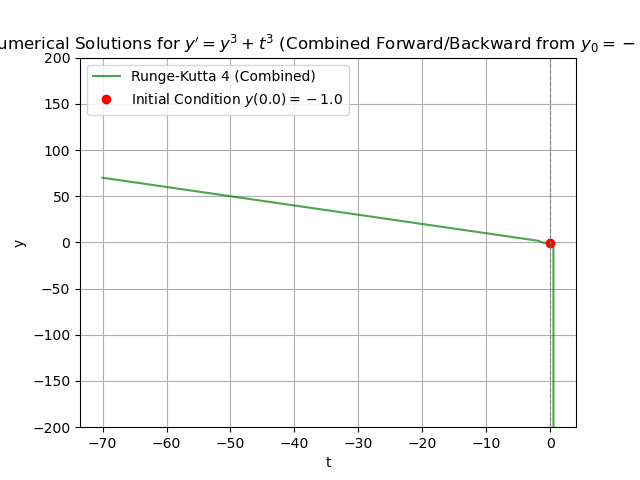
\includegraphics[width=\linewidth]{pic/kutta-1.png} % 图片宽度充满子图宽度
        \caption{y0=-1} % 为第一个图输入标题
        \label{fig:kutta-1} % 为第一个图设置一个唯一的标签
    \end{subfigure}
    \hfill % 在子图之间添加弹性水平空白,将它们推开
    % 第二个子图(中间)
    \begin{subfigure}[b]{0.3\linewidth}
        \centering
        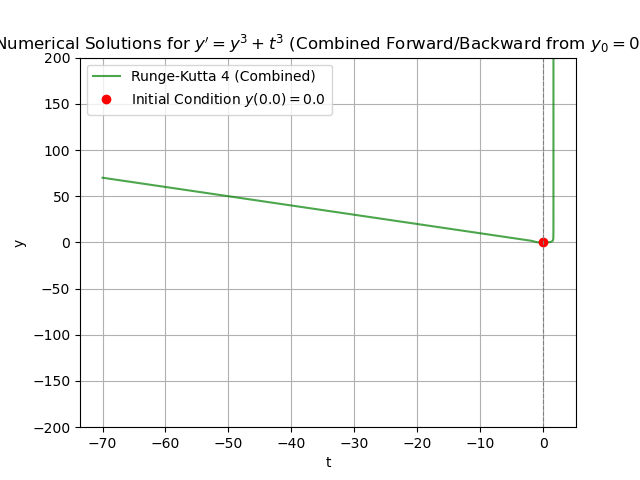
\includegraphics[width=\linewidth]{pic/kutta0.png}
        \caption{y0=0} % 为第二个图输入标题
        \label{fig:kutta0} % 为第二个图设置一个唯一的标签
    \end{subfigure}
    \hfill % 再次添加弹性水平空白
    % 第三个子图(右边)
    \begin{subfigure}[b]{0.3\linewidth}
        \centering
        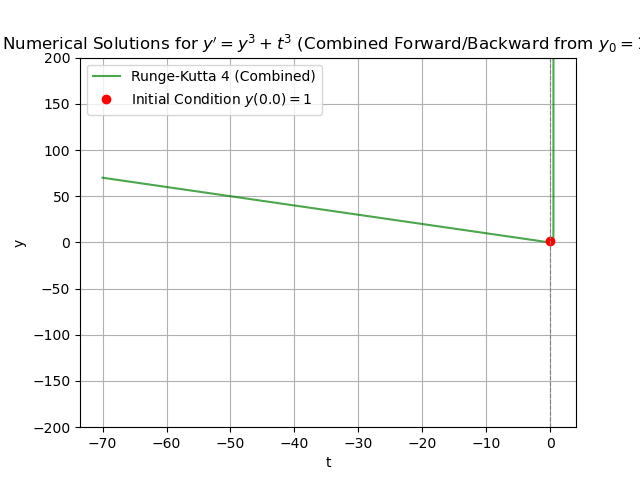
\includegraphics[width=\linewidth]{pic/kutta1.png}
        \caption{y0=1} % 为第三个图输入标题
        \label{fig:kutta1} % 为第三个图设置一个唯一的标签
    \end{subfigure}

    \caption{Runge-Kutta method} % 你可以为整个图组添加一个总标题
    \label{fig:three_kutta_images} % 为整个图组设置一个总标签(可选)
\end{figure}


% %%%%%%%%%%%%%%%%%%%%% %%%%%%%%%%%%%%%%%%%%% %%%%%%%%%%%%%%%%%%%%% %%%%%%%%%%%%%%%%%%%%


\subsubsection{Error Analysis1: Local Truncation Error (LTE)}

The Local Truncation Error (LTE) at step $n+1$ is the error made by a single step of the method, assuming the value $y_n$ at the beginning of the step is exact, i.e., $y_n = y(t_n)$.
$$ \text{LTE}_{n+1} = y(t_{n+1}) - \left( y(t_n) + h \Phi_{RK4}(t_n, y(t_n), h) \right) $$
where $h \Phi_{RK4}(t_n, y(t_n), h) = \frac{h}{6}(k_1^* + 2k_2^* + 2k_3^* + k_4^*)$, with $k_i^*$ calculated using $y(t_n)$ instead of $y_n$.
Equivalently, it is often defined as the principal error term when $y_{n+1}$ is subtracted from the Taylor expansion of $y(t_{n+1})$.



The Taylor expansion of the exact solution $y(t_{n+1})$ around $t_n$ is:
$$ y(t_{n+1}) = y(t_n) + h y'(t_n) + \frac{h^2}{2!} y''(t_n) + \frac{h^3}{3!} y'''(t_n) + \frac{h^4}{4!} y^{(iv)}(t_n) + \frac{h^5}{5!} y^{(v)}(t_n) + \Oh{h^6} $$
Substituting $y' = f$, $y'' = f'$, $y''' = f''$, etc., where $f' = \deriv{f}{t} = \pderiv{f}{t} + \pderiv{f}{y} f$, and so on (total derivatives with respect to $t$):
\begin{align*}
y(t_{n+1}) = y(t_n) + hf &+ \frac{h^2}{2}f' + \frac{h^3}{6}f'' + \frac{h^4}{24}f''' + \frac{h^5}{120}f^{(iv)} + \Oh{h^6} \label{eq:taylor_exact}
\end{align*}
All functions $f, f', f'', \dots$ are evaluated at $(t_n, y(t_n))$.


A full and detailed expansion of $k_1, k_2, k_3, k_4$ and their weighted sum $\Phi_{RK4} = \frac{1}{6}(k_1 + 2k_2 + 2k_3 + k_4)$ shows that when $y_n + h\Phi_{RK4}$ is formed, its Taylor series expansion in $h$ matches the Taylor series expansion of $y(t_{n+1})$ up to and including the term of order $h^4$.
Specifically, the expansion of $h\Phi_{RK4}(t_n, y(t_n), h)$ is:
$$ h\Phi_{RK4} = hf + \frac{h^2}{2}f' + \frac{h^3}{6}f'' + \frac{h^4}{24}f''' + C_{RK4}h^5 + \Oh{h^6} $$
The coefficients of $h, h^2, h^3, h^4$ in $h\Phi_{RK4}$ match those in the Taylor expansion of $y(t_{n+1}) - y(t_n)$.
The Local Truncation Error is then the difference:
$$ \text{LTE}_{n+1} = y(t_{n+1}) - (y(t_n) + h\Phi_{RK4}(t_n, y(t_n), h)) = \left(\frac{1}{120}f^{(iv)} - C_{RK4}\right)h^5 + \Oh{h^6} $$
Thus, the LTE for RK4 is of order $h^5$:
$$ \text{LTE}_{n+1} = \Oh{h^5} $$
This means that the RK4 method is a fourth-order method (since the LTE is $\Oh{h^{p+1}}$ for a $p$-th order method).





% %%%%%%%%%%%%%%%%%%%%% %%%%%%%%%%%%%%%%%%%%% %%%%%%%%%%%%%%%%%%%%% %%%%%%%%%%%%%%%%%%%%
% %%%%%%%%%%%%%%%%%%%%% %%%%%%%%%%%%%%%%%%%%% %%%%%%%%%%%%%%%%%%%%% %%%%%%%%%%%%%%%%%%%%



\section{Comparison for Different Methods and Different Steps}

\subsection{Analysis of Results for h = 0.1, 0.03, and 0.001}



\begin{figure}[htb] % 使用一个 figure 环境,[htb] 是位置建议符
    \centering % 将整个子图组居中(可选)

    % 第一个子图(左边)
    \begin{subfigure}[b]{0.49\linewidth} % [b] 表示底部对齐子图,宽度设置为大约页面宽度的0.3倍
        \centering
        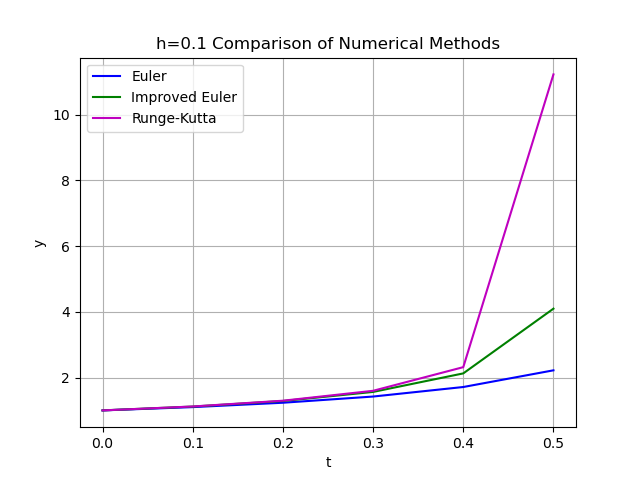
\includegraphics[width=\linewidth]{pic/comp_0.1_fig.png} % 图片宽度充满子图宽度
        \caption{h=0.1 graph} % 为第一个图输入标题
        \label{fig:kutta-1} % 为第一个图设置一个唯一的标签
    \end{subfigure}
    \hfill % 在子图之间添加弹性水平空白,将它们推开
    % 第二个子图(中间)
    \begin{subfigure}[b]{0.45\linewidth}
        \centering
        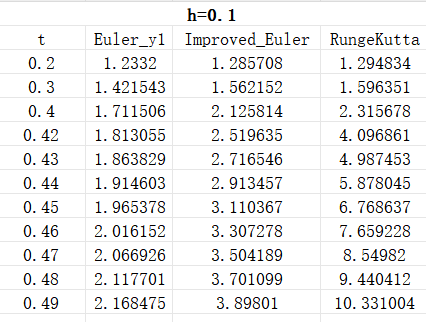
\includegraphics[width=\linewidth]{pic/comp0.1table.png}
        \caption{h=0.1 table} % 为第二个图输入标题
        \label{fig:kutta0} % 为第二个图设置一个唯一的标签
    \end{subfigure}
    \hfill % 再次添加弹性水平空白
    % 第三个子图(右边)
\end{figure}
\begin{figure}[htb] % 使用一个 figure 环境,[htb] 是位置建议符
    \centering % 将整个子图组居中(可选)

    % 第一个子图(左边)
    \begin{subfigure}[b]{0.49\linewidth} % [b] 表示底部对齐子图,宽度设置为大约页面宽度的0.3倍
        \centering
        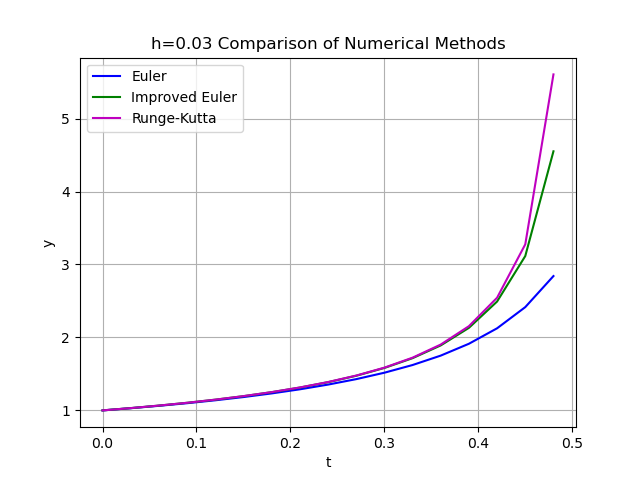
\includegraphics[width=\linewidth]{pic/comp_0.03_fig.png} % 图片宽度充满子图宽度
        \caption{h=0.03 graph} % 为第一个图输入标题
        \label{fig:kutta-1} % 为第一个图设置一个唯一的标签
    \end{subfigure}
    \hfill % 在子图之间添加弹性水平空白,将它们推开
    % 第二个子图(中间)
    \begin{subfigure}[b]{0.45\linewidth}
        \centering
        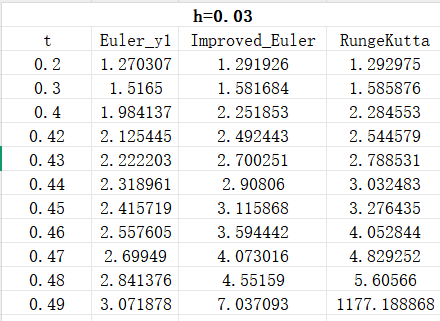
\includegraphics[width=\linewidth]{pic/comp0.03table.png}
        \caption{h=0.03 table} % 为第二个图输入标题
        \label{fig:kutta0} % 为第二个图设置一个唯一的标签
    \end{subfigure}
    \hfill % 再次添加弹性水平空白
    % 第三个子图(右边)
\end{figure}

\begin{figure}[htb] % 使用一个 figure 环境,[htb] 是位置建议符
    \centering % 将整个子图组居中(可选)

    % 第一个子图(左边)
    \begin{subfigure}[b]{0.45\linewidth} % [b] 表示底部对齐子图,宽度设置为大约页面宽度的0.3倍
        \centering
        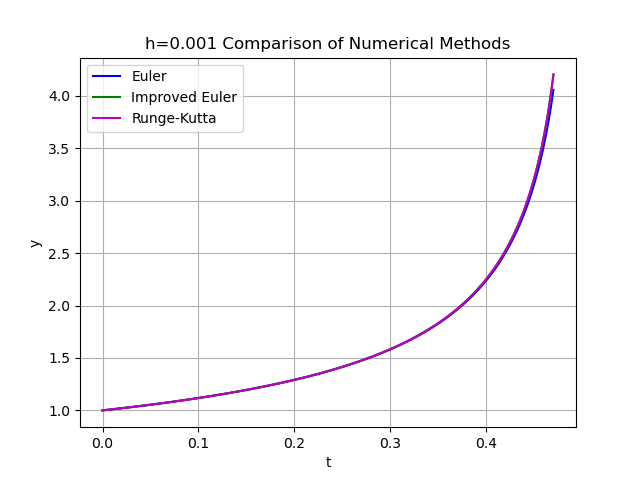
\includegraphics[width=\linewidth]{pic/comp_0.001_fig.png} % 图片宽度充满子图宽度
        \caption{h=0.001 graph} % 为第一个图输入标题
        \label{fig:kutta-1} % 为第一个图设置一个唯一的标签
    \end{subfigure}
    \hfill % 在子图之间添加弹性水平空白,将它们推开
    % 第二个子图(中间)
    \begin{subfigure}[b]{0.45\linewidth}
        \centering
        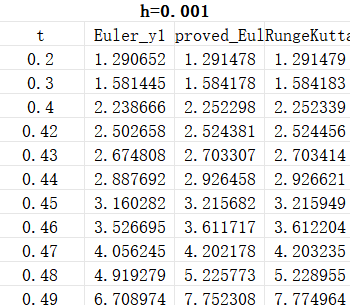
\includegraphics[width=\linewidth]{pic/comp0.001table.png}
        \caption{h=0.001 table} % 为第二个图输入标题
        \label{fig:kutta0} % 为第二个图设置一个唯一的标签
    \end{subfigure}
    \hfill % 再次添加弹性水平空白
    % 第三个子图(右边)
\end{figure}
Here, I present the variations in results for three numerical methods (Euler, Improved Euler, and Runge-Kutta) using step sizes \(h = 0.1\), \(h = 0.03\), and \(h = 0.001\). Tables and figures are provided to simplify the analysis.



The first figure corresponds to \(h = 0.1\). It can be observed that the discrepancies between the methods are quite pronounced. The Runge-Kutta method appears to yield the most distinct curve.



The second scenario (presumably with \(h = 0.03\), though not explicitly shown as a figure in the provided text) indicates that the Improved Euler method's results more closely approach those of the Runge-Kutta method. This suggests that as the step size \(h\) decreases, the accuracy of the Improved Euler method improves.



Overall, the Runge-Kutta method seems to be more accurate than the Improved Euler method, which in turn is more accurate than the Euler method.













\section{Symmetry Considerations}


\subsubsection*{1. Nullcline}

When $y' = 0$, we have $y^3 + t^3 = 0$. In the real domain, this means $y^3 = -t^3$, so $y = -t$.




Therefore, on the line $y = -t$, the slope of the solution curves of the differential equation is zero. This implies that if a solution curve crosses the line $y = -t$ (for $t \neq 0$), it will have a horizontal tangent at that point. This is an important geometric property.

\subsubsection*{2. Behavior under Transformations}
\begin{itemize}
    \item The equation is not autonomous because it explicitly depends on $t$.
    \item It is not separable.
    \item It is not a standard homogeneous equation (in the sense $y' = F(y/t)$). If we try the substitution $y=ut$, then $u't + u = (ut)^3 + t^3 = u^3t^3 + t^3$, leading to $u' = t^2(u^3+1) - u/t$. This equation is not simpler.
    \item Consider the transformation: Let $s = -t$ and $u(s) = -y(-s)$. Then $t = -s$, and $y(t) = -u(-t)$.
    Thus, $y'(t) = \frac{d}{dt}(-u(-t)) = -u'(-t) \cdot (-1) = u'(-t)$.
    Substituting into the original equation $y' = y^3 + t^3$:
    $u'(-t) = (-u(-t))^3 + (-s)^3 = -u^3(-t) - s^3$.
    Let $x = -t$. Since $s = -t$ as well, we can use $s$. So, $u'(s) = -u^3(s) - (-s)^3 = -u^3(s) + s^3$.
    Thus, if $y(t)$ is a solution to $y' = y^3 + t^3$, then $u(s) = -y(-s)$ is a solution to the equation $u'(s) = s^3 - u^3(s)$. These two equations are similar in form but not identical.
\end{itemize}
















\section{Conclusion}

In this lab report, we thoroughly explored the solutions to three initial value problems (IVPs) using both numerical and analytical methods. Specifically, we applied Euler, Improved Euler, Runge-Kutta, Picard-Lindelof iteration, and the Power Series method to solve the IVPs:


\begin{equation*}
    \text{(IVP1)} \quad y' = t^3 +y^3, \quad y(0) = -1
\end{equation*}
\begin{equation*}
    \text{(IVP2)} \quad y' = t^3 +y^3, \quad y(0) = 0
\end{equation*}
\begin{equation*}
    \text{(IVP3)} \quad y' = t^3 +y^3, \quad y(0) = 1
\end{equation*}

\textbf{Finally, we got the following for the solution's domain and behavior based on the initial condition $y_0$:}

\begin{itemize}
    \item When \textbf{$y_0 = -1$}, the function's domain extends from $-\infty$ to approximately \textbf{0.502}. The graph of the solution exhibits a shape similar to a ``check mark'' (or a hyperbola-like curve with two branches).
    \item When \textbf{$y_0 = 0$}, the function's domain extends from $-\infty$ to approximately \textbf{1.647}. The solution is strictly monotonically decreasing across its entire domain.
    \item When \textbf{$y_0 = 1$}, the function's domain extends from $-\infty$ to approximately \textbf{0.498}. Similar to the $y_0 = -1$ case, the solution's graph resembles a ``check mark'' shape.
\end{itemize}



\section{Reference}


Galaktionov, V. A. (1981). On the blow-up of solutions of the Cauchy problem for quasi-linear degenerate parabolic equations of arbitrary order. Differential Equations, 17(5), 737–743.

Arnold, V. I. (1973). Ordinary differential equations. MIT Press.
Jordan, D. W., & Smith, P. (2007). Nonlinear ordinary differential equations: An introduction for scientists and engineers (4th ed.). Oxford University Press.

Chipot, M., & Weissler, F. B. (1989). Blow-up of solutions for a class of nonlinear ordinary differential equations. Nonlinear Analysis: Theory, Methods & Applications, 13(1), 127–142.

Hairer, E., Nørsett, S. P., & Wanner, G. (1993). Solving ordinary differential equations I: Nonstiff problems (2nd rev. ed., Springer Series in Computational Mathematics, Vol. 8). Springer.

Dumortier, F., Llibre, J., & Artés, J. C. (2006). Qualitative theory of planar differential systems. Springer.




\section{Ackonwledgements}

Firstly, I'd like to say thank you to Professor Honold for assigning such an interesting task that we have learnt a lot. Then I would like to express my gratitude to all the TAs, especially TA Ren Jiashen for giving us lots' of instructions on the lab report. Thirdly, I have to say thank you to AI the Gemini, as it serves as a good coding helper for us to modify our code.​

\clearpage
\section{Appendix Coding}


\subsection{Euler Method}

\begin{verbatim}
import numpy as np
import matplotlib.pyplot as plt

# 定义微分方程
def f(t, y):
    return t**4 + y**3

# Heun 步进函数
def heun_step(f, t, y, h):
    k1 = f(t, y)
    k2 = f(t + h, y + h * k1)
    y_new = y + (h / 2) * (k1 + k2)
    return y_new

# 向前积分函数(t >= 0)
def integrate_forward(y0, t_span=(0, 5), h=0.001, blowup_threshold=1e6):
    t0, t_end = t_span
    t_values = [t0]
    y_values = [y0]
    t, y = t0, y0

    while t < t_end:
        y_next = heun_step(f, t, y, h)
        if abs(y_next) > blowup_threshold:
            return np.array(t_values), np.array(y_values), t
        t += h
        t_values.append(t)
        y_values.append(y_next)
        y = y_next
    return np.array(t_values), np.array(y_values), None

# 向后积分函数(t <= 0)
def integrate_backward(y0, t_span=(-5, 0), h=0.001, blowup_threshold=1e6):
    t_start, t0 = t_span
    t_values = [t0]
    y_values = [y0]
    t, y = t0, y0

    while t > t_start:
        y_next = heun_step(f, t, y, -h)  # 注意是负步长
        if abs(y_next) > blowup_threshold:
            return np.array(t_values), np.array(y_values), t
        t -= h
        t_values.insert(0, t)
        y_values.insert(0, y_next)
        y = y_next
    return np.array(t_values), np.array(y_values), None

# 主程序逻辑
y0_list = [-1, 0, 1]
colors = ['green', 'blue', 'orange']
h = 0.001
blowup_threshold = 1e6

plt.figure(figsize=(10, 6))

for y0, color in zip(y0_list, colors):
    # 正向积分
    t_fwd, y_fwd, blowup_time_fwd = integrate_forward(y0, t_span=(0, 5), h=h, blowup_threshold=blowup_threshold)

    # 反向积分
    t_bwd, y_bwd, blowup_time_bwd = integrate_backward(y0, t_span=(-5, 0), h=h, blowup_threshold=blowup_threshold)

    # 合并正向与反向结果
    t_total = np.concatenate((t_bwd, t_fwd))
    y_total = np.concatenate((y_bwd, y_fwd))

    # 绘图
    plt.plot(t_total, y_total, label=f"y(0) = {y0}", color=color)

    # 标记 blow-up 时间点
    for blowup_time in [blowup_time_bwd, blowup_time_fwd]:
        if blowup_time is not None:
            plt.axvline(x=blowup_time, linestyle='--', color='red', alpha=0.7,
                        label=f"Blow-up est. at t ≈ {blowup_time:.4f} (y0={y0})")

# 设置图形属性
plt.title("Solutions of $ y' = t^3 + y^3 $ using Heun's Method")
plt.xlabel("t")
plt.ylabel("y(t)")
plt.legend()
plt.grid(True)
plt.xlim(-5, 5)
plt.ylim(-10, 10)
plt.tight_layout()
plt.show()
\end{verbatim}



\subsection{Real Value}

\begin{verbatim}
import numpy as np
from scipy.integrate import solve_ivp
import matplotlib.pyplot as plt

def ode_func(t, y):
    return t**3 + y**3

# Initial conditions
y0_values = [0, 1, -1]

# Store results: {'y0': {'sol_fwd': sol_fwd, 'sol_bwd': sol_bwd, 'a': a, 'b': b}}
results = {}

# Integration parameters
t_span_limit = 20  # Max integration time in each direction (can be adjusted)
rtol = 1e-9        # Relative tolerance
atol = 1e-12       # Absolute tolerance (important for reaching asymptotes accurately)
# Using a large value for y to stop integration is an option,
# but solve_ivp often handles blow-up by itself by reducing step size until failure.
# We can check sol.status and sol.message.




for y0_val in y0_values:
    print(f"\nProcessing for y(0) = {y0_val}")


    # Forward integration
    # Integrate from t=0 to t_span_limit
    # If it blows up, sol_fwd.t[-1] is an estimate of b
    # We need to make sure t_span is large enough to pass the asymptote if one exists.
    # solve_ivp will stop if it can't proceed (e.g. asymptote)
    sol_fwd = solve_ivp(ode_func, [0, t_span_limit], [y0_val],
                        dense_output=True, rtol=rtol, atol=atol, method='Radau') # Radau is good for stiff problems

    b_asymptote = np.inf
    if sol_fwd.status == 0 and sol_fwd.t[-1] < t_span_limit : # solver might have stopped before t_span_limit due to reaching max_step or other reasons not blowup
         print(f"  Forward integration for y0={y0_val} finished early at t={sol_fwd.t[-1]} but status is 0, message: {sol_fwd.message}. This might indicate it did not blow up or needs longer t_span.")
         # If it truly didn't blow up, b is inf. Otherwise, it might be an issue with solver params or t_span_limit.
         # For this problem, blow-up is expected if y gets large.
         if abs(sol_fwd.y[0,-1]) < 1e6: # Arbitrary threshold to decide if it's not a blow up
            b_asymptote = np.inf
         else: # Assume it was on its way to blow up but stopped.
             t_last_fwd = sol_fwd.t[-1]
             y_last_fwd = sol_fwd.y[0, -1]
             if abs(y_last_fwd) > 1e3 : # Check if y is large enough for extrapolation
                 b_asymptote = t_last_fwd + 1.0 / (2.0 * y_last_fwd**2) if y_last_fwd !=0 else t_last_fwd # to avoid division by zero
                 print(f"  Extrapolated forward asymptote b for y0={y0_val}: {b_asymptote:.6f} from t_last={t_last_fwd:.6f}, y_last={y_last_fwd:.2e}")
             else:
                 print(f"  Forward solution for y0={y0_val} ended at t={t_last_fwd:.6f}, y={y_last_fwd:.2e}, y not large enough for robust extrapolation.")
                 b_asymptote = t_last_fwd # Best guess is where it stopped.
    elif sol_fwd.t[-1] < t_span_limit:  # Solver stopped early, likely due to stiffness/blow-up (status != 0)


        t_last_fwd = sol_fwd.t[-1]
        y_last_fwd = sol_fwd.y[0, -1]
        # Extrapolation for right asymptote b: b_approx = t_last + 1/(2*y_last^2)
        # This formula is for y' ~ y^3.
        # Need to be careful if y_last is small or zero.
        if abs(y_last_fwd) > 1e3: # Check if y is large enough for extrapolation
            b_asymptote = t_last_fwd + 1.0 / (2.0 * y_last_fwd**2)
            print(f"  Forward integration for y0={y0_val} stopped at t={t_last_fwd:.6f}, y={y_last_fwd:.2e}. Status: {sol_fwd.status}. Message: {sol_fwd.message}")
            print(f"  Extrapolated forward asymptote b for y0={y0_val}: {b_asymptote:.6f}")
        else:
            print(f"  Forward integration for y0={y0_val} stopped at t={t_last_fwd:.6f}, y={y_last_fwd:.2e}, y not large enough for robust extrapolation. Status: {sol_fwd.status}. Message: {sol_fwd.message}")
            b_asymptote = t_last_fwd # Best guess is where it stopped.
    else: # Reached t_span_limit
        print(f"  Forward integration for y0={y0_val} reached t_span_limit={t_span_limit} without apparent blow-up. y_final={sol_fwd.y[0,-1]:.2e}")
        b_asymptote = np.inf






    # Backward integration
    # Integrate from t=0 to -t_span_limit
    sol_bwd = solve_ivp(ode_func, [0, -t_span_limit], [y0_val],
                        dense_output=True, rtol=rtol, atol=atol, method='Radau')

    a_asymptote = -np.inf
    if sol_bwd.status == 0 and sol_bwd.t[-1] > -t_span_limit:
        print(f"  Backward integration for y0={y0_val} finished early at t={sol_bwd.t[-1]} but status is 0, message: {sol_bwd.message}. This might indicate it did not blow up or needs longer t_span.")
        if abs(sol_bwd.y[0,-1]) < 1e6:
             a_asymptote = -np.inf
        else:
            t_last_bwd = sol_bwd.t[-1]
            y_last_bwd = sol_bwd.y[0, -1]
            if abs(y_last_bwd) > 1e3:
                a_asymptote = t_last_bwd - 1.0 / (2.0 * y_last_bwd**2) if y_last_bwd != 0 else t_last_bwd
                print(f"  Extrapolated backward asymptote a for y0={y0_val}: {a_asymptote:.6f} from t_last={t_last_bwd:.6f}, y_last={y_last_bwd:.2e}")
            else:
                print(f"  Backward solution for y0={y0_val} ended at t={t_last_bwd:.6f}, y={y_last_bwd:.2e}, y not large enough for robust extrapolation.")
                a_asymptote = t_last_bwd
    elif sol_bwd.t[-1] > -t_span_limit:  # Solver stopped early
        t_last_bwd = sol_bwd.t[-1]
        y_last_bwd = sol_bwd.y[0, -1]
        # Extrapolation for left asymptote a: a_approx = t_last - 1/(2*y_last^2)
        if abs(y_last_bwd) > 1e3:
            a_asymptote = t_last_bwd - 1.0 / (2.0 * y_last_bwd**2)
            print(f"  Backward integration for y0={y0_val} stopped at t={t_last_bwd:.6f}, y={y_last_bwd:.2e}. Status: {sol_bwd.status}. Message: {sol_bwd.message}")
            print(f"  Extrapolated backward asymptote a for y0={y0_val}: {a_asymptote:.6f}")
        else:
            print(f"  Backward integration for y0={y0_val} stopped at t={t_last_bwd:.6f}, y={y_last_bwd:.2e}, y not large enough for robust extrapolation. Status: {sol_bwd.status}. Message: {sol_bwd.message}")
            a_asymptote = t_last_bwd
    else: # Reached -t_span_limit
        print(f"  Backward integration for y0={y0_val} reached -t_span_limit={-t_span_limit} without apparent blow-up. y_final={sol_bwd.y[0,-1]:.2e}")
        a_asymptote = -np.inf

    results[y0_val] = {
        'sol_fwd': sol_fwd,
        'sol_bwd': sol_bwd,
        'a': a_asymptote,
        'b': b_asymptote,
        'domain': (a_asymptote, b_asymptote)
    }

    print(f"  For y(0) = {y0_val}, estimated domain: ({a_asymptote:.6f}, {b_asymptote:.6f})")

# Plotting the solutions
plt.figure(figsize=(12, 8))
for y0_val, res in results.items():
    sol_fwd = res['sol_fwd']
    sol_bwd = res['sol_bwd']
    a = res['a']
    b = res['b']

    # Forward solution plot
    t_plot_fwd = np.linspace(0, sol_fwd.t[-1], 200) # ensure plotting up to where solver stopped
    if b != np.inf and b < sol_fwd.t[-1] + 1/(2*sol_fwd.y[0,-1]**2+1e-9): # A bit of a hack to ensure linspace is valid
        # if extrapolated b is very close to sol_fwd.t[-1] or slightly less due to numerical precision in extrapolation.
        # ensure t_plot_fwd doesn't exceed b by much if b is the true limit
        t_plot_fwd = np.linspace(0, min(sol_fwd.t[-1], b if b >0 else sol_fwd.t[-1] ), 200)


    y_plot_fwd = sol_fwd.sol(t_plot_fwd)[0]

    # Backward solution plot
    t_plot_bwd = np.linspace(sol_bwd.t[-1], 0, 200) # ensure plotting up to where solver stopped
    if a != -np.inf and a > sol_bwd.t[-1] - 1/(2*sol_bwd.y[0,-1]**2+1e-9) :
         t_plot_bwd = np.linspace(max(sol_bwd.t[-1], a if a < 0 else sol_bwd.t[-1]), 0, 200)


    y_plot_bwd = sol_bwd.sol(t_plot_bwd)[0]

    # Combine and remove duplicates, sort by time
    t_combined = np.concatenate((t_plot_bwd[:-1], t_plot_fwd)) # Avoid duplicating t=0
    y_combined = np.concatenate((y_plot_bwd[:-1], y_plot_fwd))

    # Sort by t for correct plotting
    sort_indices = np.argsort(t_combined)
    t_combined = t_combined[sort_indices]
    y_combined = y_combined[sort_indices]
    
    # Filter out extreme values if they mess up the plot too much before reaching asymptote line
    # y_combined = np.clip(y_combined, -50, 50) # Optional: for better visualization if blowup is too fast

    plt.plot(t_combined, y_combined, label=f'$y(0) = {y0_val}$')

    if b != np.inf:
        plt.axvline(x=b, linestyle='--', color=plt.gca().lines[-1].get_color(), alpha=0.7, label=f'$t={b:.3f}$ (asymptote for $y_0={y0_val}$)')
    if a != -np.inf:
        plt.axvline(x=a, linestyle='--', color=plt.gca().lines[-1].get_color(), alpha=0.7, label=f'$t={a:.3f}$ (asymptote for $y_0={y0_val}$)')


plt.xlabel('$t$')
plt.ylabel('$y(t)$')
plt.title('Solutions to $y\' = t^3 + y^3$')
plt.legend(loc='best')
plt.grid(True)
plt.ylim([-10, 10]) # Adjust ylim for better visualization of behavior near origin; asymptotes make it hard to see all details.
plt.show()

# Print summary of domains
print("\nSummary of Maximal Solution Domains:")
for y0_val, res in results.items():
    print(f"For y(0) = {y0_val}: Domain = ({res['domain'][0]:.6f}, {res['domain'][1]:.6f})")
\end{verbatim}





\subsection{Comparison Coding}

\begin{verbatim}
import numpy as np
import matplotlib.pyplot as plt

def euler(f,y0,t0,tn,h):
    t=np.arange(t0,tn+h,h)
    y=np.zeros_like(t)
    y[0]=y0
    for i in range(len(t)-1):
        y[i+1]=y[i]+h*f(t[i],y[i])
    return t,y

def improved_euler(f,y0,t0,tn,h):
    t=np.arange(t0,tn+h,h)
    y=np.zeros_like(t)
    y[0]=y0
    for i in range(len(t)-1):
        y_hat = y[i] + h * f(t[i], y[i])
        
        # 校正步骤
        y[i+1] = y[i] + 0.5 * h * (f(t[i], y[i]) + f(t[i+1], y_hat))
    return t,y

def runge_kutta(f,y0,t0,tn,h):
    t=np.arange(t0,tn+h,h)
    y=np.zeros_like(t)
    y[0]=y0
    for i in range(len(t)-1):
        k1=h*f(t[i],y[i])
        k2=h*f(t[i]+h/2,y[i]+k1/2)
        k3=h*f(t[i]+h/2,y[i]+k2/2)
        k4=h*f(t[i]+h,y[i]+k3)
        y[i+1]=y[i]+(k1+2*k3+2*k3+k4)/6
    return t,y   

def f(t, y):
    return y**3+t**3  # 定义微分方程 dy/dt = y

t0=0
y0=1
tn=0.5
h=0.001

t,y1=euler(f,y0,t0,tn,h)
t,y2=improved_euler(f,y0,t0,tn,h)
t,y3=runge_kutta(f,y0,t0,tn,h)

# yture=np.exp(t)

plt.plot(t, y1, 'b-', label='Euler')
plt.plot(t, y2, 'g-', label='Improved Euler')
plt.plot(t, y3, 'm-', label='Runge-Kutta')
# plt.plot(t, ytrue, 'r-', label='True')

plt.legend()
plt.xlabel('t')
plt.ylabel('y')
plt.title('Comparison of Numerical Methods')
plt.grid(True)
plt.show()

\end{verbatim}



\subsection{Picard Iteration}

\begin{verbatim}
import numpy as np
import scipy.integrate as integrate
import matplotlib.pyplot as plt
import math
def picard_lindelof_iteration(f, y0, t, max_iter=100, tol=1e-6):


    # 初始化解数组
    y = np.zeros_like(t)
    y_prev = np.zeros_like(t)
    
    # 初始猜测(通常为常函数 y0)
    y_prev.fill(y0)
    
    for iteration in range(max_iter):
        # 皮卡迭代更新
        for i in range(len(t)):
            # 在 t=0 处,解为初始值
            if i == 0:
                y[i] = y0
            else:
                # 积分计算:y(t) = y0 + ∫₀ᵗ f(s, y_prev(s)) ds
                y[i] = y0 + integrate.quad(lambda s: f(s, y_prev[i-1]), t[0], t[i])[0]
        
        # 打印当前迭代的 y 值
        # print(f"Iteration {iteration + 1}: y = {y}") 
        
        # 检查收敛性
        if np.max(np.abs(y - y_prev)) < tol:
            print(f"Picard iteration converged in {iteration+1} iterations")
            return y
        
        # 更新前一次迭代结果
        y_prev = np.copy(y)
    
    print(f"Picard iteration did not converge after {max_iter} iterations")
    return y


# 示例:测试皮卡迭代法
if __name__ == "__main__":
    # 定义常微分方程 y' = y,解为 y(t) = e^t

    def f(t, y):
        return y**3+t**3
    
    # 参数设置
    
    tn=1
    h=0.001


    y0 = 1.0   # 初始条件 y(0) = 1  

    s=math.ceil(tn/h) # 天花板函数

    t = np.linspace(0, tn, s)  # 时间点

    
    # 绘制不同迭代次数的解
    plt.figure(figsize=(10, 6))
    for i in range(6):
        yi = picard_lindelof_iteration(f, y0, t, max_iter=i+1)
        plt.plot(t, yi, label=f'Iteration {i+1}')
        

    
    # 绘制解析解
    # exact_solution = np.exp(t)
    # plt.plot(t, exact_solution, 'r--', label='Exact Solution')
    
    # 添加图例和标签
    plt.legend()
    plt.xlabel('t')
    plt.ylabel('y')
    plt.title('Picard-Lindelöf Iteration Convergence')
    plt.grid(True)
    plt.show()
\end{verbatim}




\end{document}

